% This is "sig-alternate.tex" V2.0 May 2012
% This file should be compiled with V2.5 of "sig-alternate.cls" May 2012
%
% This example file demonstrates the use of the 'sig-alternate.cls'
% V2.5 LaTeX2e document class file. It is for those submitting
% articles to ACM Conference Proceedings WHO DO NOT WISH TO
% STRICTLY ADHERE TO THE SIGS (PUBS-BOARD-ENDORSED) STYLE.
% The 'sig-alternate.cls' file will produce a similar-looking,
% albeit, 'tighter' paper resulting in, invariably, fewer pages.
%
% ----------------------------------------------------------------------------------------------------------------
% This .tex file (and associated .cls V2.5) produces:
%       1) The Permission Statement
%       2) The Conference (location) Info information
%       3) The Copyright Line with ACM data
%       4) NO page numbers
%
% as against the acm_proc_article-sp.cls file which
% DOES NOT produce 1) thru' 3) above.
%
% Using 'sig-alternate.cls' you have control, however, from within
% the source .tex file, over both the CopyrightYear
% (defaulted to 200X) and the ACM Copyright Data
% (defaulted to X-XXXXX-XX-X/XX/XX).
% e.g.
% \CopyrightYear{2007} will cause 2007 to appear in the copyright line.
% \crdata{0-12345-67-8/90/12} will cause 0-12345-67-8/90/12 to appear in the copyright line.
%
% ---------------------------------------------------------------------------------------------------------------
% This .tex source is an example which *does* use
% the .bib file (from which the .bbl file % is produced).
% REMEMBER HOWEVER: After having produced the .bbl file,
% and prior to final submission, you *NEED* to 'insert'
% your .bbl file into your source .tex file so as to provide
% ONE 'self-contained' source file.
%
% ================= IF YOU HAVE QUESTIONS =======================
% Questions regarding the SIGS styles, SIGS policies and
% procedures, Conferences etc. should be sent to
% Adrienne Griscti (griscti@acm.org)
%
% Technical questions _only_ to
% Gerald Murray (murray@hq.acm.org)
% ===============================================================
%
% For tracking purposes - this is V2.0 - May 2012
%\documentclass[sort&compress]{elsarticle}
%\documentclass[global,referee]{svjour}
%\documentclass[global,twocolumn,referee]{svjour}
%\documentclass[global,twocolumn]{svjour}
%\documentclass[preprint,sort&compress]{elsarticle}
\documentclass[twocolumn,]{elsarticle}
%\documentclass[10pt, conference, compsocconf]{IEEEtran}
%\documentclass{sig-alternate}
\usepackage{url}
\usepackage{balance}
\usepackage{hyperref}
\usepackage{graphicx}
\usepackage{xspace}
\usepackage{color}
\usepackage{pifont}
\sloppy

\newcommand {\pat}[1]{[{\bf \underline{Patrizio}}: {\bf #1}]}
\newcommand{\todo}[1]{\textcolor{blue}{\ding{46}~{\sf todo}~#1}}

%\newcommand{\definition}[2]{\noindent \textbf{\emph{Definition #1}} (#2)}
\newcommand{\ttransition}[2]{\stackrel{#1}{\longrightarrow^{#2}}}
\newcommand{\ntransition}[1]{\longrightarrow^{#1}}
\newcommand{\transition}[1]{\stackrel{#1}{\rightarrow}}
\newcommand{\Transition}[1]{\stackrel{#1}{\Rightarrow}}
\newcommand{\freccia}[1]{\mathop{\stackrel{#1} {\longrightarrow}} }
\newcommand{\ug}[1]{\mathop{=}\limits^{#1}_{}}
\newcommand{\barra}[1]{\overline{#1}}
\newcommand{\eqdef}{\stackrel{def}{=}}


\newcommand{\footlabel}[2]{%
    \addtocounter{footnote}{1}%
    \footnotetext[\thefootnote]{%
        \addtocounter{footnote}{-1}%
        \refstepcounter{footnote}\label{#1}%
        {\footnotesize #2}%
    }%
    $^{\ref{#1}}$%
}

\newcommand{\footref}[1]{%
    $^{\ref{#1}}$%
}

\usepackage{listings}

% colors
\definecolor{mygreen}{rgb}{0,0.6,0}
\definecolor{mygray}{rgb}{0.5,0.5,0.5}
\definecolor{mymauve}{rgb}{0.58,0,0.82}
\definecolor{light-gray}{gray}{0.85}

% listing settings
\lstset{ %
  backgroundcolor=\color{white},   % choose the background color; you must add \usepackage{color} or \usepackage{xcolor}
  basicstyle=\footnotesize,        % the size of the fonts that are used for the code
  breakatwhitespace=false,         % sets if automatic breaks should only happen at whitespace
  breaklines=true,                 % sets automatic line breaking
  captionpos=b,                    % sets the caption-position to bottom
  commentstyle=\color{mygreen},    % comment style
  deletekeywords={...},            % if you want to delete keywords from the given language
  escapeinside={\%*}{*)},          % if you want to add LaTeX within your code
  extendedchars=true,              % lets you use non-ASCII characters; for 8-bits encodings only, does not work with UTF-8
  frame=single,                    % adds a frame around the code
  keepspaces=true,                 % keeps spaces in text, useful for keeping indentation of code (possibly needs columns=flexible)
  keywordstyle=\color{blue},       % keyword style
  language=C,                      % the language of the code
  morekeywords={*,...},            % if you want to add more keywords to the set
  numbers=left,                    % where to put the line-numbers; possible values are (none, left, right)
  numbersep=5pt,                   % how far the line-numbers are from the code
  numberstyle=\tiny\color{mygray}, % the style that is used for the line-numbers
  rulecolor=\color{black},         % if not set, the frame-color may be changed on line-breaks within not-black text (e.g. comments (green here))
  showspaces=false,                % show spaces everywhere adding particular underscores; it overrides 'showstringspaces'
  showstringspaces=false,          % underline spaces within strings only
  showtabs=false,                  % show tabs within strings adding particular underscores
  stepnumber=1,                    % the step between two line-numbers. If it's 1, each line will be numbered
  stringstyle=\color{mymauve},     % string literal style
  tabsize=2,                       % sets default tabsize to 2 spaces
  caption=A program                % show the filename of files included with \lstinputlisting; also try caption instead of title
}

\begin{document}


\title{Improving interfaces customizability: an experience at Jeppesen} % of systems that communicate with different systems}

\author[CTH]{Georgios Pseiridis Pseiras, Zhenyu Zhang, Patrizio Pelliccione}
\ead{pseiras@student.chalmers.se, zhenyu@student.chalmers.se, patrizio.pelliccione@gu.se}

\author[MAL]{Romina Spalazzese\corref{cor}}
\ead{romina.spalazzese@mah.se}

\cortext[cor]{Corresponding author}

\address[CTH]{Chalmers University of Technology | University of Gothenburg\\
Department of Computer Science and Engineering,
Gothenburg, Sweden}   

%\author{\IEEEauthorblockN{Georgios Pseiridis Pseiras\IEEEauthorrefmark{1}, Zhenyu Zhang\IEEEauthorrefmark{1}, Patrizio Pelliccione\IEEEauthorrefmark{1},  %Thekla Damaschke\IEEEauthorrefmark{2}, 
%and Romina Spalazzese\IEEEauthorrefmark{3}}
%\IEEEauthorblockA{\IEEEauthorrefmark{1}Chalmers University of Technology | University of Gothenburg\\
%Department of Computer Science and Engineering,
%Gothenburg, Sweden\\
%Email: pseiras@student.chalmers.se, zhenyu@student.chalmers.se, patrizio.pelliccione@gu.se}
%%\and
%%\IEEEauthorblockA{\IEEEauthorrefmark{2}Jeppesen AB, Gothenburg, Sweden, Email: Thekla.Damaschke@jeppesen.com}
%\IEEEauthorblockA{\IEEEauthorrefmark{3}Malm\"o University of Technology, Malm\"o, Sweden, Email: romina.spalazzese@mah.se}
%%\IEEEauthorblockA{
%%Email: name@xyz.com}
%}

% conference papers do not typically use \thanks and this command
% is locked out in conference mode. If really needed, such as for
% the acknowledgment of grants, issue a \IEEEoverridecommandlockouts
% after \documentclass

% for over three affiliations, or if they all won't fit within the width
% of the page, use this alternative format:
% 
%\author{\IEEEauthorblockN{Michael Shell\IEEEauthorrefmark{1},
%Homer Simpson\IEEEauthorrefmark{2},
%James Kirk\IEEEauthorrefmark{3}, 
%Montgomery Scott\IEEEauthorrefmark{3} and
%Eldon Tyrell\IEEEauthorrefmark{4}}
%\IEEEauthorblockA{\IEEEauthorrefmark{1}School of Electrical and Computer Engineering\\
%Georgia Institute of Technology,
%Atlanta, Georgia 30332--0250\\ Email: see http://www.michaelshell.org/contact.html}
%\IEEEauthorblockA{\IEEEauthorrefmark{2}Twentieth Century Fox, Springfield, USA\\
%Email: homer@thesimpsons.com}
%\IEEEauthorblockA{\IEEEauthorrefmark{3}Starfleet Academy, San Francisco, California 96678-2391\\
%Telephone: (800) 555--1212, Fax: (888) 555--1212}
%\IEEEauthorblockA{\IEEEauthorrefmark{4}Tyrell Inc., 123 Replicant Street, Los Angeles, California 90210--4321}}





 
\maketitle
\begin{abstract}
\todo{To be refined and contextualized in the field of interoperability} This paper describes the process of handling the variability needs of a company which does not follow traditional product lines approaches and where the work of code maintenance is divided between the company and their customers. More specifically, this study focuses on improving the customizability of interfaces used for data transmission through different system, where misinterpretations can occur leading to problematic communication.
We document the guidelines for decision making and suggest ways for future work. We pushed the prototype on the company's code repository, ready to be used by their employees and hopefully be proven useful. 
We hope that the findings of this study could support the customization endeavors of companies of similar technical contexts. 
\end{abstract}

\begin{keyword}
Software customization, Variability Handling, Product Lines, Interoperability, Maintainability
\end{keyword}

%\IEEEpeerreviewmaketitle

\section{Introduction}

\todo{To be refined and contextualized in the field of interoperability}    
Handling variability is crucial for a company which places great emphasis on mass customization. 
Software variability is defined as the ability of a software system or artifact to be changed, extended or configured for use in a specific context. 
%As the variability is improved, the system can be easier customized (Svahnberg, Gurp, Bosch 2001). 
Variability is a leading aspect of success in software engineering but at the same time a dominant reason for complexity augmentation~\cite{vonRhein2016}. % (Rhein et al. 2015). 
%To exploit the benefits of variability, requirements between different stakeholders need to be addressed and different software solutions should be proposed. There is not a single software package which could satisfy all customers. Customization is therefore often presented as a solution to the needs of the different customers (Weiss \& Schweiggert 2013).



%\section{Purpose and objective}

%There is a risk of problems occurring between different systems due to their inability of to interpret correctly the given parameters.
%Therefore, to mitigate this, e
Effective variability management is required to enclose the activities needed to explicitly manage variability and handle the dependencies among the various software artefacts~\cite{Schmid2004}. %(Schmid \& John 2003 p260).


In the concrete case of the Jeppesen Company, located in Gothenburg, Sweden, in each installation, their crew planning
and tracking system is put into a unique system context that needs to exchange information
with a varying set of other systems from different vendors. The timely and correct
information exchange is crucial for the ability of the system to provide the expected services
with expected quality. Especially for a tracking system, interoperability problems
with surrounding systems can lead to severe impact on the airlines operation

Due to the high degree of variation which is required, interface development has so far been the domain of customization. 
These interfaces define the interpretation of the airline data. In the past, each airline had their own customer specific interfaces to communicate with the company's systems. This is what we refer to as the {\bf ``old system}". The company is currently striving to introduce standard interfaces. In this way they are expecting to move away from customer specific interfaces and impose a standard behaviour which will be followed by all airlines. This is what we refer to as the {\bf ``new system}". However, in the avionics field, it is a common phenomenon for different customers to use their own interpretation of otherwise well-defined standards and thus violating the imposed standard behaviour. 

%Software product line engineering techniques cope with the high demand of variation among their products. Software product lines define a family of products which share commonalities and variations with each other and can be viewed as a family of products (Bosch Capilla \& Kang 2013). Product line techniques suggest ways to minimize the costs of development, maintenance and evolution of the software products (Svahnberg, Gurp \& Bosch, 2001 p2). The software companies are responsible for their products during all the life-cycles.
%
%
%There is a significant area of research about handling software variability where a considerable amount
%of different methods have already been proposed. These methods suggest patterns,
%theoretical frameworks and tools, mainly in the context of software product lines. These methods work under the assumption that the maintenance of the software systems is being done completely by the company's side and that the required variation will live for very long.

To make things even more complex, part of the system's code of Jeppesen %However, this is not the case for Jeppesen, as part of their system's code 
is maintained by their customers. After the
company delivers their systems, they lose control over customer specific source code. Their clients are responsible for partial code maintenance and compatibility of their systems. Therefore, the risk of incorrect interpretation of the provided parameters is high when one of the systems in the whole landscape is updated or replaced.


%This study aims to support the customization efforts in a company which does not follow traditional product line engineering techniques. We asses and analyze the requirements, compare them with existing solutions and define whether they fit in our case. The outcome of this thesis are the guidelines to support future decision making for the customization needs of similar contexts based on the acquired knowledge, accompanied by solid reasoning.

The goal of this work is to provide guidelines to 
%guidelines to 
support future and possibly unpredictable customization needs of a software system whose code maintenance is divided between the company and its customers. 
%support future decision making for the customization needs triggered by future and possible new clients. 
%similar contexts based on the acquired knowledge, accompanied by solid reasoning.

%\section{Research questions}
%We have defined two research questions to determine a decision making strategy. These research questions are as follows:\\

%\textbf{RQ1:} What are the variability needs and what are the limitations of the interfaces?\\\\
In order to suggest a method we needed first to understand the nature of the required variation of the interfaces.
%This research question's aim was to let us understand the context and provide a basis to design a method to address the variability needs. 
We therefore had to understand, why different airlines interpret well-defined standards in different ways, what causes faulty communication between different systems, which parts of the standard are still open for interpretation and how did the company so far managed the variability inside these interfaces. %To answer these questions, we interviewed experts inside the company about a specific standard interface. 
%To gain an insight of the company's technical context we performed semi-structured interviews, a group interview and code analysis.


 %To get the state-of-the-art of existing methods for variability handling, we performed literature review. The interviews were recorded, transcribed and analyzed further. 
The knowledge gained %from the literature was documented and 
has been then used to suggest a conceptualized solution.
Finally, the solution has been implemented and validated.

\todo{Guidelines}

\todo{Context of the software center, interoperability project}

\todo{Summary of the paper}

%We defined two research questions which served as the main guidelines of the research. In this way, we expected to come closer to the research goal by answering them.
%We later performed a trade-off analysis of the existing methods found in the generic literature. The purpose was to give solid argumentation of which method was more suitable in the problem under investigation. 
%We later proceeded to develop a prototype and evaluate it.  
%After the analysis phase was over, we tried to answer the second research question which was:  \\

%\textbf{RQ2:} What are the guidelines to support the customization efforts of a software system whose code maintenance is divided between the company and its customers?
%\\
%Therefore, we defined the guidelines to support the customization efforts of a software system whose code maintenance is divided between the company and its customers.

%This research question is concerned with providing the outcome of the thesis. Having obtained the context of the problem based on the first research question, we tried to suggest guidelines to effectively increase the customizability of their systems. These guidelines would be based on solid reasoning and evaluated to ensure the degree to which it is successful in facilitating the customization needs of the company under study and other companies with similar technical context.


%\raggedbottom






%\section{Scope and limitations} 
%
%This thesis focuses on the variability handling issues in the technical context of Jeppesen, located in Gothenburg, Sweden. Thus the conclusions of this study might not be applicable to other companies. Additionally, the main focus is placed on improving the customizability of the new system although we interviewed stakeholders working in the old system as well. However, the new system was supporting only one customer by the time this study took place.
%It is therefore hard for our method to be integrated right away since the possible emerging use cases are not well known right now. 
%
%The basis of the study was placed on a single, rather complex interface where several aspects are affected at the same time. It is concerned about timetable information and although it is standardized, airlines still interpret it differently with each other. Each field in the standard is translated into semantics which systems can be understood my Jeppesen's system. However, since some fields are open for interpretation, the processing of the semantics could lead to incorrect results.
%
%
%Later during this study, we decided to expand the scope to another interface to investigate whether the suggested method for the first interface could be replicated to a similar context.
%This is the operational messages interface which can be considered as family of standards. Due to limited time, for this interface we took a more theoretical approach.

%\section{Method} 
%
%The methodology followed the guidelines of design research as described in (Vaishnavi \& Kuechler, 2004). We tried to first understand the problem and create knowledge by implementing our conceived idea.  
%To gain an insight of the company's technical context we performed semi-structured interviews, a group interview and code analysis. To get the state-of-the-art of existing methods for variability handling, we performed literature review. The interviews were recorded, transcribed and analyzed further. 
%The knowledge gained from the literature was documented and used to suggest a conceptualized solution.
%
%We defined two research questions which served as the main guidelines of the research. In this way, we expected to come closer to the research goal by answering them.
%We later performed a trade-off analysis of the existing methods found in the generic literature. The purpose was to give solid argumentation of which method was more suitable in the problem under investigation. 
%We later proceeded to develop a prototype and evaluate it.  


%\section{Outline of the thesis} 
%
%\noindent {\bf Structure of the paper:} this paper is structured as follows. In chapter 2 we present general information about the company and the systems they develop. In chapter 3 we present the key concepts of software customization and variability handling that this thesis is focused on and discuss the related work.
%In chapter 4 we present the methodology we followed to deal with the variability problem under investigation.
%In chapter 5 we discuss about the main variation points, the main indicators which influenced our decision making and a trade-off analysis of the main realization mechanisms.
%In chapter 6 we discuss the development process while in chapter 7 we present the evaluation of our approach and the guidelines for future decision making. In chapter 8 we state the threats of validity. The study concludes in chapter 9 and suggestions for future work is presented.

\section{Background}

Boeing was founded on July 15, 1916 by William Boeing and is the world's leading aerospace company\footnote{The Boeing Company: \url{http://www.boeing.com/}}. %\todo{(Boeing, 2016)}. 
This study took place in one of their subsidiary companies called Jeppesen founded in 1934\footnote{Jeppesen - Transforming the Way the World Moves: \url{http://ww1.jeppesen.com/index.jsp}}. They offer a diverse set of products such as navigation charts, planning tools and crew management systems. This study focuses on the last. In this section we discuss the background of the company, presenting an overview of their crew management systems, the interfaces we studied and the avocado model.

%VALE PRWTA TO CREW MANAGEMENT SYSTEMS
\subsection{Crew management systems}

An enormous amount of airlines expenses comes from the costs of moving crew. Jeppense's office in Gothenburg specialises in providing crew management solutions to airlines so as to increase the crew productivity. The planning process is very complex and consists of a number of different stages:

\begin{itemize}
\item {\em Manpower process}: %the general number of crew members, along with the required qualifications is defined. This can be considered as defining 
anonymous work-blocks for crew personnel are defined together with required qualifications. These work-blocks %where they 
should be filled by real people later on and the companies can decide who should be hired, promoted, who needs training and how the leave should be divided.
\item {\em Pairing:} set of flight legs, which start and end in the same destination. This is a sophisticated process where a large number of factors should be taken into consideration.  When the crew comes back, the pairing is finished. 
There are a lot of restrictions such as the hours the crew can work, how many continuous days they are allowed to work, the different workforce laws of the country they come from to name a few. 
\item {\em Rostering:} 
%The next process is called rostering and it is about 
assigning actual personnel so to define the %. The rosters can be viewed as the 
actual work schedules. Again, here there are lot of restrictions. For example, a trip going to Brazil requires at least one crew personnel who can speak Portuguese. What is more, a crew member might wish to take a few days off and therefore another crew member should replace him or her for. Sometimes crew cannot work together or they should work together. 
\item {\em Crew tracking stage:}
%Finally, there is the crew tracking stage. This is where 
the company tries to solve problems when they arise. For example, a crew member who got sick in the middle of his or her assigned trip has to be replaced by another member who is on standby in this city.  
\end{itemize}

Valid and consistent information exchange between different systems is crucial for the optimization system to provide the best results. However different airlines have different customization needs. Consequently, their systems vary with each other. This imposes a threat for the information interoperability as there is a risk for misinterpretations of the exchanged data.  



\subsection{Standard interfaces }

International Air Transport Association (IATA)~\cite{IATA} provides support for most airline companies throughout the world. The IATA manual defines the structure and behaviour of both interfaces of the study. We used the issue of March 2011 for the study. 


\subsubsection{SSIM interface}
The Standard Schedules Information Manual (SSIM) defines the interface which is complied to the IATA regulations. It is used from airline companies to produce schedule data in the form of timetable information. The airline companies generate an SSIM file which is then distributed to multiple recipients such as airline reservation systems, timetable agencies, air traffic control authorities and so on~\cite{IATA}.
Jeppesen systems use these files for crew and fleet management, with a strong emphasis on optimization of crew pairing, rostering and tracking. The need for the consistency of the data is therefore considered highly important in order to create valid and efficient solutions.



The interface under investigation has been selected because it is  well-known by the people in the company and it is well-defined by the IATA manual. However it contains a number of variability points. This means, there are parts of the standard which are open for interpretation that the interface should be aware of. Therefore, it was considered a good candidate to provide a basis for this research, where the outcome could be replicated to other similar interfaces as well. 

The manual provides explicit formatting rules to define the interface's syntax. Each byte in the syntax has its own meaning and corresponds to one of the supported fields. It should be noted that the company's systems do not read all the fields, since some of the optional fields such as meal service, have no impact on crew planning and are therefore discarded.


\subsubsection{Operational messages interface}

The second interface is about the operational messages, which could be considered as a family of formats. They are concerned with information regarding amendments of flight schedules, deviations from original schedules and aircraft movements. 
The information are being exchanged between airlines, aircraft and schedule aggregators~\cite{IATA}. % (International Air Transport Association, 2011). 


An identifier is placed at the beginning of the message to differentiate between each format. Information for permanent changes to basic schedules are transmitted through the Standard Schedules Message (SSM). Modifications of schedules are defined through the Ad-Hoc Schedules Message (ASM). Aircraft Movement Messages (MVT) are concerned with messages regarding departure, arrival and delay of a flight which were produced manually. Aircraft Initiated Movement Message (MVA) are concerned with messages of the same nature as with MVT but produced by the aircraft itself~\cite{IATA}. % (International Air Transport Association, 2011).


The manual provides guidelines for specifying a diverse set of actions for each of these formats, in the form of sub-messages. These actions, for example, can define behaviour for inserting a new flight designator, update information of existing flights and change of existing routing information. Each of these sub-messages are specified in a similar fashion as with the SSIM's case; each byte corresponds to a field which contain data for messages between the aircraft and the airport. Not all the messages are being used by each airline. 

\subsection{The old and the new system}
In this section we present the difference between the old and the new system for when it comes to parse SSIM files. 

\subsubsection{The old system}
The variability binding takes different approaches in the two systems. The old system provides a form that allows its users to define many parameters when they wish to import the raw data from SSIM files, giving them the capability to configure the system in run time. These parameters correspond to one more flags of the tool. Some of them are taken from the input form, some are taken from the configuration files. The files are then converted to a specified format and handled by the same component of the tool.

The original code, which was written in C language, was closely following the IATA format and it was expected to be used in the same way by all the customers. In reality, the algorithms had to be adjusted to accommodate more customer specific requirements. 
%This resulted in an immense main function, with many global variables, that is extremely complex, 
This resulted in an extremely complex code which was 
hard to read and manage, as described by the company's experts. Although it works correct and satisfies the expected functional requirements, it is hard to maintain as there is a high risk of problems occurring when the system is updated.

\subsubsection{The new system}
The new system divides the work of interpretation and logic handling between the adaptor and the back end, as shown in Figure~\ref{fig:newSystem}.  

\begin{figure}[h]
\centering
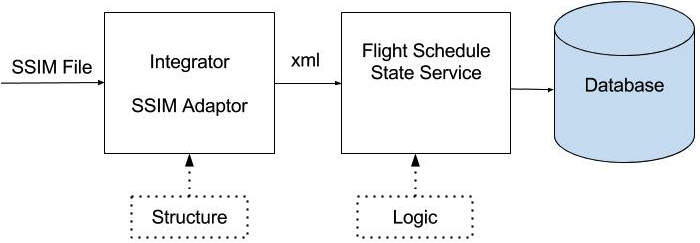
\includegraphics[width=\columnwidth]{figure/Figure2.png}

\caption{ General overview of parsing an SSIM file and storing it in the database}
\label{fig:newSystem}
\end{figure}


The aim is to have separation of concerns between these two components. The SSIM file is generated by an airline company and used as an input to the integrator. The integrator, consecutively, uses an adaptor to define the structure for the SSIM standard in XML form. The ``Flight Schedule State Service" component imports this XML file and applies some well defined computations to handle the given semantics accordingly. Finally it stores in the database the converted information. 

The integrator's code of the new system is wrote in Python. 
%was originally written in Java. However, during our analysis phase, the company changed the programming language to Python. Although the logic stayed somewhat the same, we had to perform additional code analysis and change our documentation appropriately. For example, the class diagrams had to be redrawn. Based on these diagrams we later placed our proposed solution. 
%An important aspect of our decision making was, for each variability point, which of these two components had to be selected. Whether or not it was a structural or logical problem. 
%Finally, it should be mentioned that the 
Within the old system variability is managed at run-time while in the new system the variability is bound at build-time. This means, the old system allows the users to change the interpretation of the parsing of SSIM files by providing an input form containing a number of parameters. However, the new system was initially designed and built to manage customer specific use cases. Later, when they changed the technology from Java to Python, they still provided plug-in scripts which extent the system's core architecture that address customer specific issues. 

%\subsection{The avocado model}
%The Avocado model demonstrates how the company develops its products. This Avocado Model is shown in Figure~\ref{fig:avocadoModel}.
%
%\begin{figure}[h]
%\centering
%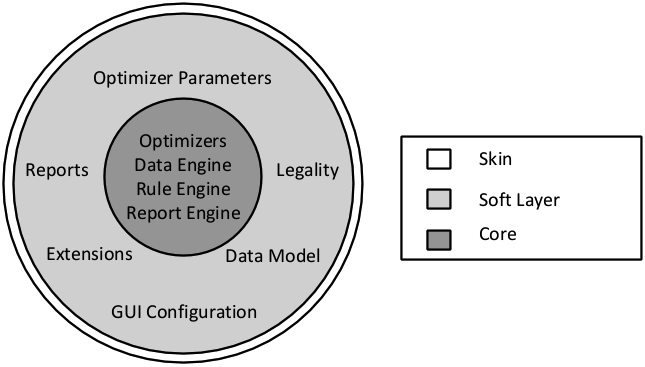
\includegraphics[width=\columnwidth]{figure/figure11.png}
%\caption{ The Avocado model. }
%\label{fig:avocadoModel}
%\end{figure}
%
%
%The core part consists of functionality that is the same to all of their customers. For example, all the optimization algorithms are embedded in the core. The translation of SSIM information to semantics is also inside the system's core. \\
%Then, there is the soft layer that surrounds the core. This layer contains the business logic and it can be different from customer to customer. For example, union contracts are different between the United States and Europe. Another example is how the graphical user interface is displayed from customer to customer. Even the translation of the SSIM can be modified to adhere to an airline's needs.
%This layer can be modified by the airlines companies alone, or with the help of Jeppesen engineers. The configuration can be done by utilizing a domain specific language developed by the company as well as by writing Python scripts which do not require the system to be recompiled. The soft layer therefore varies for each airline. Jeppesen does not have control over this layer after their system is delivered. It is up to the airlines to maintain it. \\
%Finally, there is the skin, which is the outer layer of the avocado. This is where the system allows its users to define parameters. For example, how many days off in a month can a crew member have. 









\section{Research Method}

This study follows the guidelines for design research in information systems, as presented by~\cite{Hevner2004}. % \todo{(Vaishnavi \& Kuechler, 2004)}. 
In this section we describe the steps we followed in order to propose our suggestion and collect feedback. 

In summary, the steps we followed were as follows: 
 \begin{enumerate}
  \item Understand the context of the problem by performing semi-structured interviews and code analysis.
  \item Capture, document and analyze the extracted information.
%  \item Perform literature review to explore available solutions from the state of the art.
  \item Provide trade-off analysis for each variability point.
  \item Conceive a solution and realize a prototype for showing the idea.
  \item Evaluate by collecting feedback from key stakeholders in the company
  \item Iterate this process, refine the method, expand the scope and re-evaluate
 \end{enumerate}

%\subsection{Research Method}
We first had to understand the context of the problem. Then, we explored the current available solutions and select the optimum by providing the reasoning behind. This enabled us to suggest a way to solve it by designing a prototype. We then proceeded to evaluate our suggestion based on the feedback of the company's stakeholders. Based on that we further refined our method. Additionally,  to assess whether or not our approach could be applied to another similar context, we used the findings of the first iteration to suggest a way for another interface. Feedback from experts was once again collected and documented. 

%Figure~\ref{fig:method} shows the process steps we followed.
%
%\begin{figure}[h]
%\centering
%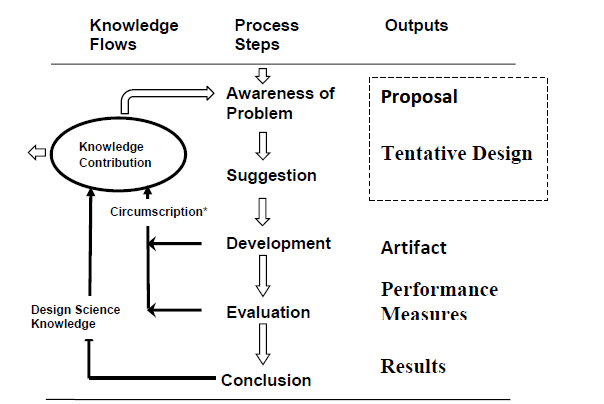
\includegraphics[width=\columnwidth]{figure/Figure1.png}
%\caption{The process model for design research. Taken from~\cite{Hevner2004}}
%\label{fig:method}
%\end{figure}


%
%\subsection{Awareness of the problem}
%Initially, the focus was placed on the SSIM interface only. After concluding the first iteration with the evaluation we decided to expand the scope to a second interface. Due to time constrains and the required effort to build the required components, the second iteration had a more theoretical approach.  
%\subsubsection{Interviews}

\noindent {\bf Awareness of the problem:} In an attempt to extract the knowledge which was dispersed in several stakeholders of the company, we conducted a number of semi-structured interviews. In this way, we gained an insight about the context of the SSIM interface, the customization procedures and other relevant technical information. The identification of right interviewees was considered fundamental for the study. %We wanted to extract as much relevant information as possible. 
For this reason we focused on stakeholders who worked with interfaces, either as developers or by interacting with customers. %Some interviewees had a hard time to give us relevant information that we needed but they helped us by pointing some other person who could help us more during our analysis phase. 
%We only kept the information we believed was relevant for our study, after the interviews were complete. Irrelevant information for example could be about the difficulty to understand error reports when the parsing of SSIM files fail, as it had nothing to do with improving the customization of this interface.
Those stakeholders were in total twelve, as shown in Table~\ref{tab:stakeholders}. 

 
%\begin{itemize}
%\item
%% Hokan
%A developer who worked in the implementation of the SSIM parser in the old system.
%
%\item
%%anton, phillipe, camtcha 
%Three software engineers involved in the development of the new system, including the SSIM parser.
%%Robert
%\item A system's expert involved in the production of the new system who also gave us an insight of the new system's architecture.
%
%%Thekla
%\item A system Architects of the Core Technical Development, involved in the development of the old system but also provides support in the new system's architecture.
%
%%IO product owner
%\item A process consultant who also plays the role of the Product Owner of the new system.
%
%%Stefan
%\item A system expert who is also a Subject Matter Expert in pairing systems and with vast experience in the old system.
%%Henrik Magnus
%\item Two service managers from the Service center, who come in contact with clients.
%%Hans Andreason
%\item A systems expert from the Implementation Department, who engage in customization and delivery procedures, sometimes with the help of customers.
%%Hans Eriksson
%\item A Business Consultant involved in premarket and benchmark activities
%
%\end{itemize}
%%\hfill 

\begin{table}[h]
\begin{center}
{\small 
\begin{tabular}{|p{.15cm}|p{1.3cm}|p{5.5cm}|}
\hline\hline
{\bf \#} & {\bf Role} & {\bf Reason/Expertise}\\
\hline
1 & Developer & Worked in the implementation of the SSIM parser in the old system\\
\hline
3 & Software engineer & Involved in the development of the new system, including the SSIM parser\\
\hline
1 & System expert & Involved in the production of the new system who also gave us an insight of the new system's architecture\\
\hline
1 & System architect & Part of the core technical development, involved in the development of the old system, provides support in the new system's architecture\\
\hline 
1 & Process consultant & Plays the role of the product owner of the new system\\
\hline
1 & System expert & Subject Matter Expert in pairing systems and with vast experience in the old system\\
\hline
2 & Service manager & Contact person with clients\\
\hline
1 & Systems expert  & Part of the implementation department and engages in customization and delivery procedures, sometimes with the help of customers\\
\hline
1 & Business Consultant & Involved in premarket and benchmark activities\\
\hline\hline
\end{tabular}}
\end{center}
\caption{Interviewed stakeholders}
\label{tab:stakeholders}
\end{table}


%The interviews followed a semi-structured approach by preparing questions beforehand. 
Each interview was planned for at least thirty minutes. However, some of the interviews took longer, with a maximum time of one hour and twenty minutes, as we allowed the interviewees to elaborate more based on topics that were considered relevant to the study. 
All the interviews were recorded and later transcribed for further analysis. 

Additionally, in an attempt to mitigate the risk that we might have missed some important aspect or that the questions might have been misunderstood by the experts and also to ensure the consistency of our findings a group interview also took place. In the group interview engineers from both the new and old system were involved and we allowed them to discuss with each other for each point that was raised. The total time of the group interview was approximately sixty minutes.

The main focus of all interviews was placed on identifying the variability issues within the SSIM interface. However, to further facilitate our understanding of the general context that this interface operates in, other issues were also taken into consideration. Discussion about the high-level architecture of the new system as well as the general demonstrations of the company's business goals and challenges took place during this phase.

%\subsubsection{Code and document analysis}
\noindent {\bf Code and document analysis:} 
In addition to the interviews we performed also an analysis in deep of the code and of the available documentation. 
The aim of this study is to allow the new system's integrator to become more configurable. We therefore considered code analysis of both the old and the new system's source code as an essential part of our study. Main focus was placed on the translation process of the SSIM files, containing raw data, to semantics which the company's system can understand. We analyzed the code both of the old and the new system. Especially in the new system, code analysis was essential for the development of the prototype as it required understanding of the classes, their methods, their data structures and their dependencies. 

For the code analysis of the old system an engineer who had worked a lot on the SSIM integration part was also involved. We used screen capturing software to record the code analysis in order to facilitate its documentation. In this way we could look into the code multiple time with the expert's commentary and grasp the issues of the old approach. He explained how the code was written and refactored in the past, the challenges they have faced and the causes of complexity. Moreover he proceed to demonstrate the functionality of the system by running some test cases. 

The code analysis of the new system was mostly done manually by us. However, support of the engineers was provided by answering our questions and providing short explanation of the reasoning behind their implementation. We have also been involved in the new system's team meetings where we kept notes of their discussions. These meetings discussed mostly the architectural aspects of the new system's integrator. 
%Finally, analysis of relevant company documentation was applied. 

These documents included the 2011 version of the IATA standard manual, architecture diagrams, official manuals and tutorials of both systems. Especially the manual of the IATA standard helped us a lot to understand the code of both systems and based on that we got a grasp of the customer specific use cases that have appeared in the past or might appear in the future.


%\subsection{Literature review}
%In order to get a background of the research problem, a set of research papers, journal articles and dissertations have been selected. The core focus was placed on the variability
%management and handling, software customization and design patterns. Our purpose is to adopt a method based on the state-of-the-art variability handling methods which we consider relevant to the company's technical context. In the previous chapter we discussed the related work based on the literature review. 
%We started by reviewing a systematic literature about variability in software systems done by (Galster et al. 2014). We read the summary of variability mechanisms in product lines by (Lee \& Hwang 2014) and also reviewed the referenced papers. We adopted definitions presented in (Svahnberg, van Gurp \& Bosch, 2001), a paper which is cited many times. We also followed their taxonomy for variability realization techniques in (Svahnberg, van Gurp \& Bosch, 2005) which is also referenced by many other papers. 
%The keywords we used to obtain references from various digital libraries were closely related to variability management. Literature related to variation point models, patterns for software variability, variability modelling and software customization were selected. The appropriateness of the selected literature is evaluated by
%reading the abstract and introduction, the proposed tools and frameworks and their implementation or the overview of the method and finally the conclusion of the study.
%In the related work chapter we presented the main methods we discovered. 

%\subsection
\noindent {\bf Trade off analysis and development}: 
%blabla gia trade off. 
We were looking for a solution which would adhere to the requirements of the company's stakeholders. We therefore wanted a solution with as minimal effort to implement as possible. During the trade off analysis we looked through the available methods in the literature; we assessed their applicability on the company's context and their expected strengths and weaknesses. 
We documented the results of the analysis and discussed the different methods with stakeholders in the company. Based on their feedback we decided which of the methods were more appropriate for interface customization and we proceeded to develop a prototype. 
In section~\ref{sec:approach} we present the trade off analysis for each method. 

%\subsection{Development}

%Having concluded with the trade off analysis, we picked a method and went on to design a prototype. The initial design was on the core Java implementation. However, when the company changed to Python, we went a step back and tried another approach. 

%The idea was to observe whether or not we could support the customization of the use cases we found through the interviews. Each use case was dealt in isolation and we observed whether or not our suggestion could support them.
\noindent {\bf Solution construction}: 
Having concluded with the trade off analysis, we picked a method and went on to design a prototype. The idea was to observe whether or not we could support the customization of the use cases we found through the interviews. Each use case was dealt in isolation and we observed whether or not our suggestion could support them. 
The development was done in a test-driven development approach. We started by writing a test case which represented a use case and let it fail. We then wrote code which would make the test case pass. The prototype included a separate python module which would inherit and overwrite parts of the system's core code. The core code was left intact. 



%\subsection{Evaluation}
\noindent {\bf Evaluation}: 
After the completion of the prototype we proceeded to evaluate it. We wanted to get early feedback to see whether or not our method is aligned with the company's customization needs so as to decide how we would continue.  For this purpose, we invited experts from the company to collect initial feedback. The stakeholders involved were a system expert of the new system and a service manager from the service center department. The system expert was the person who wrote the parser's code in Python. The person from the service center was selected because he comes in contact with customers. 

The evaluation started by asking permission to record the evaluation. We later used slides and performed a live demonstration of our prototype. We asked their opinion of the strengths and weaknesses of our approach. We transcribed and analyzed their feedback. Based on it we would then proceed to refine our method further. 

The final evaluation took place after the refinement of our original approach. The stakeholders involved were engineers of the new system, one of the new system's architect, an architect from the core development product, a line manager and a stakeholder from the implementation team. The presentation included slides which gave an overview of our work, the problem at hand and the flow of logic of how we concluded to our results. After the presentation we encouraged the employees to give us their opinion. We stressed the importance of why they think this way. We encouraged them to elaborate on the reason they think our approach is good or bad and to discuss with each other.


\section{Towards effective variability handling}\label{sec:approach}


The first step towards an effective way to handle variability is by understanding it. This is also required if we want to answer the first research question regarding the variability needs and limitations. For each variability point, we identify the variable item, why different airlines have different needs and which are the required variants, as suggested by~\cite{Pohl2005}. % (Pohl, B�ckle,  Linden. 2005 p60). 

In this section we present the main variation points of SSIM and Operational Messages interfaces. We then present an overview of how the old and the new system parse SSIM files. Finally, we discuss the indicators which influenced our decision making and provide a trade-off analysis of variability realization mechanisms.


\subsection{Variation inside standard interfaces}
\subsubsection{Main Variation Points of SSIM}

The results of the analysis phase led to the identification and grouping of the main variation points of the investigated interface. We use the term variation point to describe the parts of the standard which are open for interpretation from customer to customer. The system needs to be aware of these fields and their required variants, providing a mechanism to handle the possible use cases. 

Some of the issues of more technical nature were not considered as variation points. These issues were mainly related with the inability of some customers to produce proper SSIM files complying with the IATA standard. For example, a customer might include four bytes in a field that is meant to contain only two, ruining the syntax for the rest of the fields. It is then up to the customer to fix the syntax of the corrupted files and resend it again. 
%pes oti eixame provlima na kanoume extract ta UC

During our interviews we observed that the various stakeholders had some difficulty to remember all the use cases which appeared in the past. During the group interview, the significance of each variation point was discussed. The general feeling was that the standard should be the same for everyone and there should be no room for interpretation. However some stakeholders strongly believe that this can hardly be the case and it is very likely that airlines will impose their own use cases, as it happened before. By the time our study started, the new system was supporting only one customer and the requirements for the next ones were not known. 


We summarize the main variation points of the SSIM in Figure~\ref{fig:SSIMvariability}.

\begin{figure}[h]
\centering
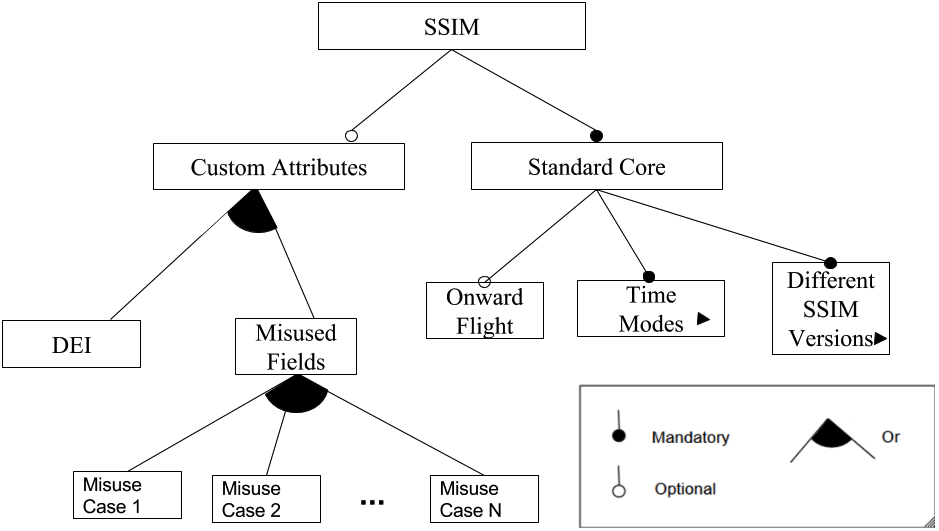
\includegraphics[width=\columnwidth]{figure/figure12.png}

\caption{ Main SSIM variability points using feature diagrams}
\label{fig:SSIMvariability}
\end{figure}



The SSIM standard contains two main parts. The standard core part which contains the fields shared by all the customers.
We found three variation points inside the standard core.
The first one is an optional field for the onward flight information. The second one is the different time modes. Lastly, there can be different versions of SSIM followed by different airlines. We illustrate further the variants of the variation points for the time modes and different SSIM versions in Figure~\ref{fig:SSIM}. %figure 5.2. 

The second part is about extending the standard through custom attributes where the customers can add more functionality.  Custom attributes can take the form of data element identifiers (DEI) which are defined by the IATA manual. They can also take the form of misused fields, where customers violate the syntax in some way.


\begin{figure}[h]
\centering
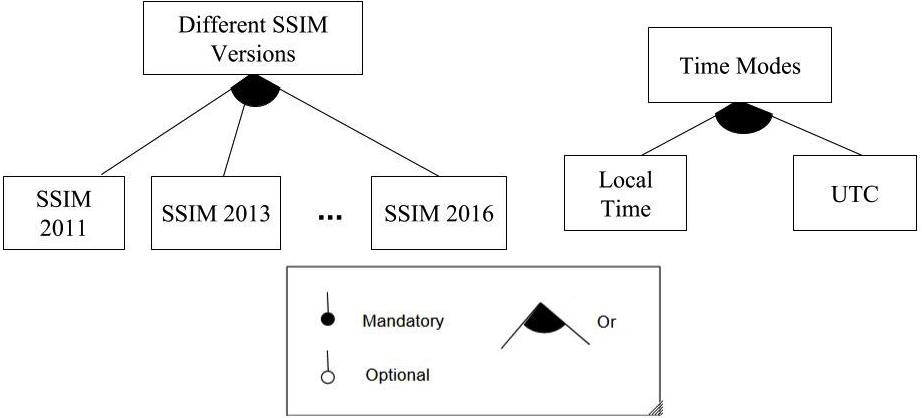
\includegraphics[width=\columnwidth]{figure/figure13.png}
\caption{ Different SSIM Versions and time modes}
\label{fig:SSIM}
\end{figure}



Depending on the IATA manual issue which an airline uses, different SSIM versions can exist. Some airlines might even use very old versions. 
Time modes can be either in Local Time or UTC. In the following sub sections we include more details for each variation point.


\subsubsection{Data element identifiers }
We begin with the Data Element Identifiers (DEI) as the first identified variation point. These can be used to extend the SSIM interface. This way customers can address their individual and distinct needs. DEIs take the form of an integer in a specific field inside the interface. Another string field corresponding to this DEI contains information to address an airlines specific requirements. The DEIs are described by the IATA manual and each integer has a different meaning. Currently there were only four DEIs supported inside the core code of the new system, as their total number can be a few hundred different cases. 


\subsubsection{Misused Fields }
Moreover, there can exist customer specific use cases which can not be handled by the use of DEIs.The system needs to know how it should handle each customer's individual case.  An example of such case is code-share issues, where an airline might wish to replace the subsidiary  carriers with the main carrier. Another example is the departure time shown to the customers and the actual departure time of the aircraft. This might occur because in some airports the passengers are being transported with buses to the aircraft, so there might be a few minutes variation. However, from crew planning perspective the aircraft time is what is important. As a last example, some customers use the flight service type, such as cargo only, in the field that is meant for the flight suffix. Finally, there could exist a case where an airline might want to use a field inside the SSIM interface which is usually not read by Jeppesen's systems. Therefore the system should be aware of this case and act accordingly. 
During the group interview all the stakeholders agreed this was the most urgent variability point.



\subsubsection{Different SSIM versions}
In addition to the custom attributes, different SSIM versions exist. The IATA standard releases a new version of their manual twice a year. During our investigation we used the 2011 version as a reference. Airlines whose systems use a very old version might not be compatible with the newer ones. Throughout the different versions, lots of fields have new meanings. Some unused or empty fields start being used. Some of the fields that the company normally does not read might be required by some customers. However, according to some interviewees in the group interview, this is  rarely a problem as it is very rarely changed in a major way. Furthermore, some clients might have a completely new use case which results on a modified version of the SSIM standard.    

\subsubsection{Time modes }
Another issue is related with the time mode an airline company is using. More precisely, for the date of operation of each flight leg can be specified either in UTC or in Local Time. Although the IATA standard states that the time shall be in UTC, some customers still might want to store it in local time because this was the time format their systems were using. It should be noted that the handling of this issue is responsible for a significant percentage of the old system's code complexity, according to engineers in the company. As an example, a flight from an American airport can take place late at night. If the airline company sends the time in Local Time, the day of operation is different in UTC time because it is a different day in Europe. This can cause confusion, especially since the day of operation for each flight should be unique according to the IATA standard.

\subsubsection{Onward flight}
Finally, stakeholders raised the issue of an optional field containing information about the onward flights. These flights are concerned with the next leg flown by the same aircraft. The information about these flights can either be missing, or it can be included and still not be consistent. The system should be able to handle these cases as this information is necessary for planning purposes. 





\subsubsection{Main variation points of Operational messages interface }
We identified four variation points for the operational messages interface. 
The first variation point is concerned with whether or not the aircraft rotations need to be updated.  Different airlines have different scheduling process. In this interface, the company can choose to either update the onward aircraft rotations by performing an action or keep the same information provided by the SSIM. If the airline actually wishes to update the onward information, functions which swap flight legs or assigning new pointers in the rotations can be called. 

The next variation point is about the time mode for the date of origin. The manual for the operational messages says the time should be in UTC, but some airlines especially in America still use local date of origin because it is easier to keep unique. However, the time obtained from the SSIM interface can still be in Local Time. As an example, a flight starting late at night in USA which uses Local Time, appears to be the next day in Europe. The system therefore needs to know how to properly adjust the date accordingly. 

Another variation point is about the diversions from original schedule. When a flight leg can not land to the original arrival station it might have to land to another airport. This can occur, for example, because of harsh weather conditions. The follow up messages might be different between airlines. The aircraft might have to go back to its original destination, or continue to the next destination. The variation lies on the assumption of what the aircraft should do, as long as not further message arrives or opposite, for what situation additional messages are expected

Finally, the last identified variation point is concerned with the reliability of the different sources the system gets messages from. If an airline company has an internal consolidation system, then this requirement is not needed at all. An example of different sources reliability would be the messages for the actual and estimated time of departure. For actual time of departure the system would typically trust more the messages sent from the aircraft, while for estimated messages it would trust those sent from the airport.  




%\subsection{The old and the new system}
%In this section we present the difference between the old and the new system for when it comes to parse SSIM files. 
%
%\subsubsection{The old system}
%The variability binding takes different approaches in the two systems. The old system provides a form that allows its users to define many parameters when they wish to import the raw data from SSIM files, giving them the capability to configure the system in run time. These parameters correspond to one more flags of the tool. Some of them are taken from the input form, some are taken from the configuration files. The files are then converted to a specified format and handled by the same component of the tool.
%
%The original code, which was written in C language, was closely following the IATA format and it was expected to be used in the same way by all the customers. In reality, the algorithms had to be adjusted to accommodate more customer specific requirements. 
%%This resulted in an immense main function, with many global variables, that is extremely complex, 
%This resulted in an extremely complex code which was 
%hard to read and manage, as described by the company's experts. Although it works correct and satisfies the expected functional requirements, it is hard to maintain as there is a high risk of problems occurring when the system is updated.
%
%\subsubsection{The new system}
%The new system divides the work of interpretation and logic handling between the adaptor and the back end, as shown in Figure 5.3  
%
%\begin{figure}[h]
%\centering
%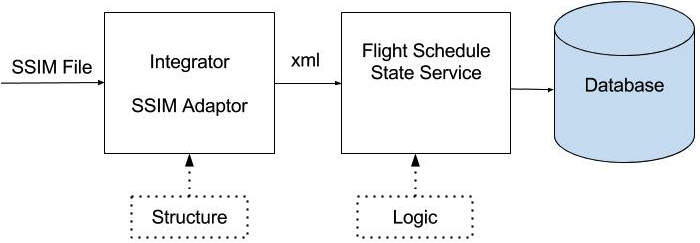
\includegraphics[width=\columnwidth]{figure/Figure2.png}
%
%\caption{ General overview of parsing an SSIM file and storing it in the database}
%\end{figure}
%
%
%The aim is to have separation of concerns between these two components. The SSIM file is generated by an airline company and used as an input to the integrator. The integrator, consecutively, uses an adaptor to define the structure for the SSIM standard in XML form. The ?Flight Schedule State Service? component imports this XML file and applies some well defined computations to handle the given semantics accordingly. Finally it stores in the database the converted information. 
%
%The integrator's code of the new system was originally written in Java. However, during our analysis phase, the company changed the programming language to Python. Although the logic stayed somewhat the same, we had to perform additional code analysis and change our documentation appropriately. For example, the class diagrams had to be redrawn. Based on these diagrams we later placed our proposed solution.\\ 
%An important aspect of our decision making was, for each variability point, which of these two components had to be selected. Whether or not it was a structural or logical problem. 
%Finally, it should be mentioned that the old system is managing variability in run time while in the new system the variability is bound in build time. This means, the old system allows the users to change the interpretation of the parsing of SSIM files by providing an input form containing a number of parameters. However, the new system was initially designed and built to manage customer specific use cases. Later, when they changed the technology from Java to Python, they still provided plug-in scripts which extent the system's core architecture that address customer specific issues. 
%\raggedbottom

\subsection{Indicators for selecting a method}\label{sec:indicators}

There is a number of indicators that greatly influences our decision making for selecting one of the available methodologies. We tried to suggest a way to handle each variation point independently. The first step to manage each of these, according to the guidelines provided by the taxonomy of~\cite{JillesVanGurp2001}, %(Svahnberg, van Gurp \& Bosch, 2005 p708), 
is to identify the variability and where it is needed. These are the variation points which we identified during the context's analysis phase. 

The next step, based on these guidelines, is to constrain the variability. A variation point which can include a significant number of possible alternatives, is often preferable not to include all of them in the first version of the system. The system should include those that are more likely to appear and allow the possibility to accommodate more in the future~\cite{JillesVanGurp2001}. % (Svahnberg, van Gurp \& Bosch, 2005 p710).  

Additionally, the current architecture plays a significant role to our decision making, as there is currently a single fully-working instance of the system. There is a separation of concerns between the parsing of the data and the actual logic handler. We therefore need to decide, for each variability point, which component should we use for our implementation. The technology of the system also is taken into consideration along with its strengths and limitations.

The next step, according to~\cite{JillesVanGurp2001} % (Svahnberg, van Gurp \& Bosch, 2005 p714) 
is to populate the variant feature, that is, how the variant should be created and integrated inside the existing components of the system. The population can either be implicit or explicit. Implicit population means the system does not recognize the available variants. Explicit population means the system actually provides functionality to support the required variants. As an example taken from the authors of the taxonomy, an \textit{IF-Statement} is implicit population, since the system can not usually add more \textit{ELSE-Statements} during run time. This decision indicates when should the binding time of the variants be done. This can either be in build or run time.

In the old system, some of the variants were supported during run time system. The users were able to select the variants they wish during the system's operation through the provided input form when they were loading the SSIM files. There was also a build time option where users could parse a configuration file along with the SSIM files to specify their additional requirements. These files included code which corresponded to the DEIs, as specified in the IATA manual.
In the case of the new system though, the engineers prefer a build time solution. However, run time variability might be supported in the future for some of the variation points. 

Another very important factor is the decision of who is expected to populate a variant feature by writing or compiling code~\cite{JillesVanGurp2001}. % (Svahnberg, van Gurp \& Bosch, 2005 p715). 
The end users can still make use of the customization layer to write their own scripts.
After all, Jeppesen allows their customers to customize their system according to their needs through domain specific language and by Python scripts. As mentioned before, the customers are able to customize the system on the customization layer. For compiling and building the system, it is up to the engineers of the company.

Finally, a decision should be taken of how to bind the variants. This can either be done internally or externally~\cite{JillesVanGurp2001}. % (Svahnberg, van Gurp \& Bosch, 2005 p717). 
Internal binding means that the system provides the required functionality for a particular variation point. External binding means the system makes use of an external entity that implements the binding, such as an external module, another system, an external tool or even a person.


\subsubsection*{Summary of indicators}

\pat{requirements for the solution} The indicators are based on the feedback of the engineers of the new system during the analysis phase of our study. 

Below we present the summary of the indicators:\\

\begin{itemize}



\item The collection of variants should be populated \textit{implicitly}. The company does not wish to include or maintain customer specific code. Therefore, the system needs to include code to only satisfy a particular customer's use cases.

\item The system binds the variability during build time, where it is designed and handed over to the customer.

\item When it comes to who needs to write the required code, the customers are expected to modify the system to handle their variability needs in the form of Python scripts.

\item This means that the functionality should be bounded \textit{externally}. 


\end{itemize}




\section{Development and implementation of proposed solution}

In order to explain the idea of our solution we developed a prototype. 
%The aim of our study is to create knowledge by attempting to solve a concrete customization problem. %In this way, we tried to answer the second research question, that is, in which way we could increase the system's customizability. 
%We proceeded to develop a prototype so as to show the idea. 
We started with the custom attributes variation point, which was considered as the most urgent from the company's stakeholders. 
In this section we present the steps we followed during the development phase of our study. %The discussion of the feedback is described in the next chapter.


%\subsection{Java implementation}
%The integrator's code was initially entirely written in Java. Since there was only one customer, there were not any known customer specific requirements for the new system. Our initial assumption was that the system would require run time binding, because this was the way it worked in the old system. Based on the taxonomy of (Svahnberg, van Gurp \& Bosch, 2005 p735-737) and the figure 5.5
%we considered two code-level realization techniques. The first one was run time variant component specializations and the second was variant component implementations. These techniques make use of design patterns in code level to manage variability. The reason we choose these techniques was based on the indicators which stated that the binding should be done in run time, the collection of variants should be explicit while the system provides internal functionality. 
%
%Our original suggestion was to apply behavioural design patterns. Behavioural patterns are linked with the assignment of responsibilities between objects and the handling of diverse algorithms. These patterns favour object composition over inheritance (Gamma et al. 1995 p221).
%
%For the case of custom attributes, we tried to to make use of the strategy pattern. As originally presented in (Gamma et al. 1995 p315), this pattern defines a family of algorithms, encapsulates each one and makes them interchangeable. Strategy lets the algorithm to vary independently from the clients that use it. In this way we expected that we could encapsulate the required behaviours for the different misuse cases inside separate classes.
%
%We tried to design the parser in a way to make use of this pattern by creating sub-classes. These sub-classes would include the different algorithms for managing the different misuse cases. In this way, we tried to separate the parts of the application that vary and the parts that belong to the core of the product, that need to stay the same. We consider the handling of customer specific use cases as different algorithms that affect the behaviour of the system.
%
%Our assumption was that not many misused cases would appear since this was the general impression we obtained during the group interview. Otherwise, should their number become too big it could lead to class explosion, resulting in increased system complexity. 
%
%
%
%
%\subsection{Change of technology}
%
%The company changed the programming language of the integrator from Java to Python. This was done in order to handle the parsing of multiple SSIM files at the same time. This functionality was also present in the old system. 
%\\
%There is now a main core application written in Java. This application calls python scripts which support the translation of the SSIM input to XML. Furthermore, the company provides customer specific scripts. These scripts inherit and overwrite parts of the core implementation. This way they adjust the system to adhere to each of their customer requirements. The customers can also edit these scripts since there is no need to recompile the system. 

\subsection{Existing solution} %Code analysis results }
%The main logic stays somewhat the same with the Java approach. 
The core of the integrator uses python modules to define the structure and the general parsing rules. The module is called \textit{ssim.py} which is included in the \textit{std\textunderscore interfaces \textunderscore adaptors} core package.

As shown in Figure~\ref{fig:classDiagram}, there is a distinction between the core and customer specific layer. The core part, which is on the right of the figure, handles the generic issues of transforming the SSIM into an xml file. The left part includes scripts which handle the concrete issues that are specific for a specific airline company. The DEIs are handled inside the \textit{ssim.py} inside the package \textit{std\textunderscore interfaces \textunderscore adaptors} of the core part. The IF-statement which handles the data element identifiers is relatively small when our research was performed but it could still significantly increase in size in the future.

The airline specific module \textit{ssim.py} is included inside the \textit{as\textunderscore adaptors} package of the customer specific layer. The script inherits and overwrites parts of the super class it adheres to, without the use of interfaces or abstract classes. The size of this script is limited to less than fifty lines of code and handles two concrete use cases. 
This approach binds the variability in build time. There is clear separation between the core and varying customer specific solutions. In this way, the company increases the maintenance of the system since only the additional scripts need to be maintained which cause no ripple effects to other modules. 


\begin{figure*}[h]
\centering
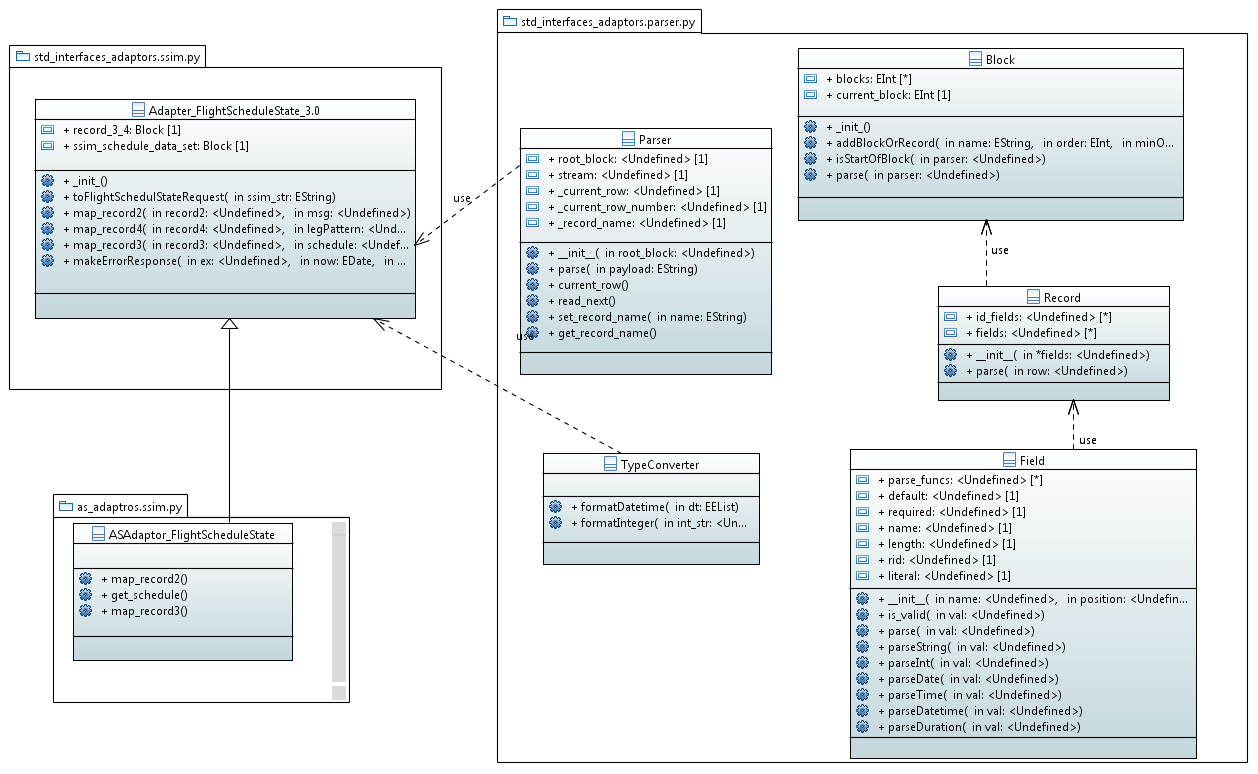
\includegraphics[width=1.0 \textwidth]{figure/figure8.png}

\caption{Existing solution}
\label{fig:classDiagram}
\end{figure*}


\subsubsection{Issues of the existing solution}

The approach the company is following is quite efficient. The core stays the same for all customers and they are responsible for editing scripts to customize it further. They are also responsible for their maintenance and keep it compatible with their systems; Jeppesen loses control over the code. 

During our study we raised some issues. Hard-coded conditions were included inside the customer specific scripts. The follow-up question was whether or not we could somehow reuse parts of the code. In this way, we hoped to decrease the amount of code required to handle use cases which appear more than once.


Another issue we raised was to what extent could the airlines write quality code by themselves. After all, they need to focus on airline related problems than programming related problems. Writing a Python script requires understanding of the system's core code as well as writing test cases to ensure the code provides the expected results.


Finally, there was the issue concerning what would happen when all the company's customers migrate to the new system. The maintenance is done by the airlines side which means they are responsible to keep compatible their systems. 
According to some stakeholders who come in contact with customers, they receive support calls when their customers can not figure out how to fix their systems and even sometimes they complain that they receive too much code to maintain.  

By the time this study was performed, there was only one airline supported in the new platform and the company was talking with the second customer. The goal of this study was to look further ahead and suggest a way to mitigate emerging risks.  

\subsubsection{Suggested approach}
%Contrary to our initial approach, we decided our method should 
Our approach aims for build time binding and implicit collection of variants and external functionality. This decision was made by asking some practitioners within the company whether run time binding was needed. %This question was asked to the developers of the new system after the Java-to-Python transition was made. 

Based on the \todo{above indicators}, we looked into different techniques of the taxonomy, such as the variant component specializations and optional component specializations~\cite{JillesVanGurp2001}: % \todo{(Svahnberg, van Gurp \& Bosch, 2005 p733-735)}: %These choices follow the figure 5.5. and based on the indicators we discussed in section 5.3, we selected two methods as follows:

 \begin{figure*}[!t]
 \centering
 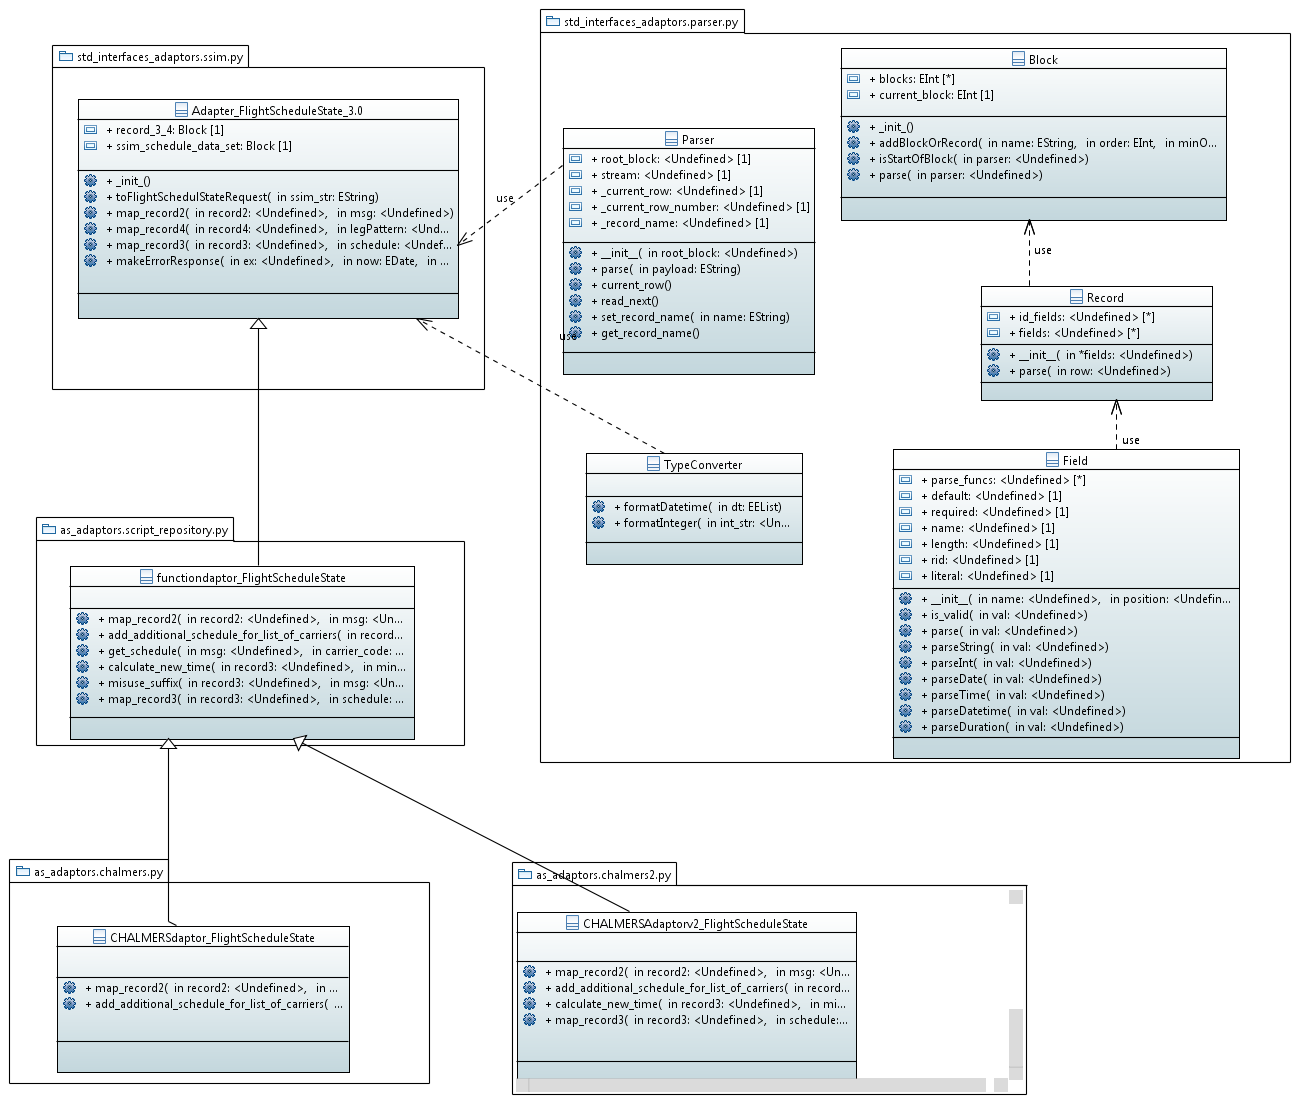
\includegraphics[width=1.0 \textwidth]{figure/figure9.png}
 
 \caption{Approach using a script repository in Python}
 \label{fig:ourApproach}
 \end{figure*}


\textit{Variant component specializations} suggest a method where a particular component is adjusted to addresses different variability issues. This is realized by creating a number of independent classes and selecting those who are required to be included for each case. 

\textit{Optional component specializations} is about including or excluding the relevant behaviour of a component for each case. This can be realized by developing a separate class which encapsulates the optional behavior~\cite{JillesVanGurp2001}. % \todo{(Svahnberg, van Gurp \& Bosch, 2005 p733-735)}.
 

Inspired by those methods, our new approach suggested a grouping of the recurring methods in a separate module. This module would inherit and overwrite parts from the core implementation but the customers would only need to import this module on their scripts and use the available methods by simply parsing parameters. 

The main idea was to support the customization by allowing the users to select among a set of provided functions instead of customizing those functions.
In this way, we hoped to reduce the code duplication for handling these case as we expect that only the provided parameters will change in the future. We also hoped we would increase the understandability of the system. 

\subsection{Development process}
To achieve this, we developed a new Python module which contains methods to handle misuse cases. We called this python module as \textit{script\textunderscore repository.py} and we created two children scripts, \textit{chalmers.py} and \textit{chalmers2.py} that made use of the provided scripts to handle a number of concrete use cases. In Figure~\ref{fig:ourApproach} we present the class diagram of our approach.






In order for the script repository to define algorithms for each use case, different parts of the core implementation had to be taken into consideration, such as the provided methods and data structure definitions. 


Our prototype's was built in a test driven development approach; we first wrote a test case, we let it fail and we proceeded to write code to make it pass. For this reason, we have written a new file explicitly for writing our own test cases which were satisfied by the modules  \textit{chalmers.py} and \textit{chalmers2.py}. Moreover, we have written a test case that only makes use of the core implementation in order to make sure we have not altered anything in this part and that the core is working as expected. 

The \textit{script\textunderscore repository.py} is the module which needs to be maintained and extended. The children modules only needed to call these methods and provide the appropriate parameters. 

\subsubsection{Example use cases}
To show the idea behind our approach, we tried to support a few use case. Two of these use cases were making use of a certain airline's requirements, which the engineers have solved but in a hard-coded way. These use cases were related with replacing the codes of the subsidiary carriers to to the main carrier and the inclusion of additional schedules to these subsidiary carriers. Our approach would only require the customer to import our module and call these methods with the corresponding parameters.

We also tried to solve some conceptualized use cases, based on what we discovered during our interviews in the analysis phase.
The first use case had to deal with the time variation of the departure time. If the departure time had to be adjusted a few minutes, the script would again only require to import our repository and call the corresponding method with the appropriate parameters. 
Finally, we tried to handle the misplacement of the service type suffix, when some airlines use the operational suffix instead of service type field. We handled this case in the similar fashion as above, by calling the corresponding method. In this case, however, no parameters were required.

Our approach follows our initial assumption that not too many customer specific requirements would emerge. Should this be the case, there could be an explosion of methods. Additionally, these methods are only viable if they are required from at least more than one customer. In the next chapter we provide a more detail discussion about this approach. 


\subsubsection{The rest of the variation points} 
We have observed that not all of the issues can be handled with the same method. For each individual variation point a decision had to be made on which part of the system it should be handled. More precisely, for each variation point we had to decide whether it could be solved as a structure or logic issue. Therefore, the adapter or the logic-handler modules would had to be selected respectively. 

The focal point of was placed mostly on the different misuse cases. We have investigated further of how to handle the rest of the variation points to decide whether or not it could be handled with our approach or in a different way. Our findings suggest that not all points could be handled with our suggestion. 

Local time and UTC time adjustments require special logic handling. The algorithms responsible for this handling have already implemented in the logic component of the new system. The only requirement is that the input XML file provides the correct semantics to define whether the time is Local Time or UTC time. In this way, there is no need to adjust the system for each customer as it is able to handle all cases.

Similarly, the onward flight has been handled in this way. The algorithms to handle inconsistent or missing onward information is handled for all customers in the same way inside the logic part of the system. According to company's experts, there could still be a way to provide a generic method to handle this issue. However, the required parameters would probably be too many and the time needed to investigate how this could be implemented would probably be immense. We therefore decided that this variation point is out of the scope of our thesis.

We have verified that the DEIs are being effectively handled in the core part of the system. After all, DEIs follow are defined by IATA standard and do not misuse the SSIM syntax. We have validated this functionality by writing tests and compare the expected output with a given input based on SSIM files we obtained from the company. 

For special cases of certain DEI numbers, an IF-Statement in the core part suffices. This method is also described in the taxonomy of~\cite{JillesVanGurp2001} %\todo{(Svahnberg, Gurp, Bosch 2005 p739)} 
as \textit{Condition on variable} which intent is to include functionality to support multiple operations. There are currently only a small subset of all the possible integers a DEI can have, as not all of them are required by all the customers right now. For each new customer who actually wants to use a new DEI, a new ELSE-Statement would be added. Therefore the overall IF-Statement could become potentially big and since it is currently included in the core part of the parser, it would might add up to its complexity. If this should be the case, we suggest to include this IF-Statement into a separate module and call it through the main core implementation by parsing the corresponding DEI. 


Finally, when it came to handle the different versions of the SSIM interface, we observed that this could be handled in a similar way as with the misuse cases. If there are major differences between the supported version and the version an airline is using, it is implied that there is a need for adjustment. Company's experts have also agreed that this case could be considered as a special case of syntax misuse.
As an example, a field of an older version could have a different meaning than the current version. Should this be the case, then a method from our repository could be called and adjust the system in the appropriate way. 

However, during our investigation we have observed that if a customer wants the system to read a field that the company usually does not support, this can not be simply handled with our approach. We tried to write a method to handle this issue but it was futile as the system would require to be rebuilt and recompiled to become aware of this field. Our conclusion, supported by the developers of the new system, was that this can only be solved manually by the company's side.


\subsubsection{Operational messages variation points} 

We tried to discuss ways to deal with the variation points of the operational messages interface. The suggestions include high-level methods to handle variability in this context. The aim to see whether or not the suggestions made for the SSIM interface could be replicated in this context. The discussion involved the system architect of the new system. Evaluation of this discussion was performed during the last presentation in the company which also involved engineers of the new system. Everyone seemed to agree with these suggestions. We assume that the company would follow the same logic of separation of concerns, where the raw input is translated to XML semantics and is being handled in the backend. 

For the updated aircraft rotations variation point, there is a need to indicate whether or not the flight legs need to be updated. The decision whether or not to update these rotations could therefore be considered as a structural issue. Depending on an indicator, the corresponding function could be called.  
By default it would assume that there is no need to update the rotations at all. The functions would be written by Jeppesen engineers but the selection could be done by the customers. Therefore the algorithms could be part of the core and encapsulated in the backend. The customers could simply edit a script to include an indicator to call these functions.

In a similar fashion the date of origin could be managed. A flag in the translated xml file could indicate that a system is using local time. The recalculation is done in the backend part of the core. Therefore it is shared among all customers and the functions are written by the company's engineers. The selection among the functions could simply be done by the customers. 

The reliability of the different priorities is a rather complex variation point. It could be done entirely in the customization layer and it would require explicit functions which would overwrite parts of the core. The system could prepare support for priority handling, either in the core or in the customization layer.

Finally, the diversions variation point could be viewed as a structural issue. The point is to define which would be the next flight leg. This could be handled by editing a script and calling the corresponding function and parsing parameters. This is intertwined with the repository of scripts suggestion of this study. However, if the functions are proven to be rather hard to replicate because of vast numbers of parameters, documentation and coding standards could facilitate this purpose.
\section{Validation and Results}\label{sec:results}

Our suggestion was heavily influenced by the company's customization needs. Therefore, our suggested method needed to be easy to introduce, implement, maintain and extend. In this chapter we  discuss the results of our findings by discussing the strengths and weaknesses of the method and the knowledge gained from this endeavour. 

\subsection{Validation}

The use cases handled by the prototype provided some satisfying results. In order to use the script repository, an airline company only needs to import our module and call one of the available methods by parsing parameters. The total amount of lines of code a customer needs to write in order to use a method from the repository approximately four or five, including the import of our module in the beginning. Including an additional method requires at maximum three extra lines of code.
The company's current approach required approximately ten to fifteen lines of code for developing a customer specific method which inherits and overwrites part of the core implementation.

Additionally, we developed our own test cases to validate that we were getting the expected results. The test cases compared a string of raw data input in the form of SSIM format to a string of the expected XML file. Their customers do not require to write the test cases by themselves. We have included commented test cases in a package where they can adjust fields of the SSIM and XML accordingly. In this way we hope that we can guarantee that our methods will work.

Finally, there is no need for airlines to understand how the core's code or the methods inside the script repository work. The algorithms and data structures needed to handle these use cases as they have already been implemented from the company's side.

\subsection{Evaluation}
After the completion of our prototype, we proceeded to evaluate it by asking for feedback from company's stakeholders. Initially, we invited two key stakeholders to evaluate our approach. Based on this evaluation, we went on to discuss with a systems architect for refining our method. In this way we identified the guidelines for decision making which we describe in a later subsection on this chapter. After that, we invited stakeholders to our final evaluation where we presented our work, our suggested method for both SSIM and Operational Messages interfaces, the decision making process and ideas for future work. 


\subsubsection{Preliminary feedback}
We performed a presentation with two key stakeholders of the company to evaluate our suggested method. The first stakeholder was the developer who wrote the Python code of the integrator in the new system. The second stakeholder was a person who works in the service center of the company. 
We used slides to show the idea behind our approach. These slides also included code parts which compare our method with the current implementation. The evaluation was recorded and later transcribed. %We present the main points from the feedback we got in this section.


%% ( ---- )WEAKNESSES
%At first, our approach received was treated with scepticism. The main reason was that they did not intend to maintain customer specific code at all. According to the first stakeholder, it is up to the clients to edit Python scripts to modify the system according to their needs, especially since Python language does not require to recompilation of the system.  
%
%The second reason was whether or not they could reuse the methods to handle customer specific issues. According to the first stakeholder, this approach would add up to the complexity of their system's modules. There were currently no concrete evidence to support the argument that customer specific methods could be reused. The reason was the use cases were unknown to them since the new system supported only one customer at that moment.   
%
%Additionally, he argued that this repository of methods could become potentially large and hard to be used; the clients might feel lost of which method they need to use, especially if some methods had to be used together.
%The second stakeholder then also stated that he was sceptical for the degree on which the methods could be reused. As an example, he talked about the code sharing issue; whether it could be handled in the same way for multiple airlines or each airline had their own interpretation. 

%On the other hand, our approach received some positive feedback as well. The person from the service center stated that our 
On the positive side the two stakeholders judge judge that the approach simplifies the system's use from the client
perspective. He argued that their clients are airlines and not IT companies.
By following our approach they would enable their customers to focus on actually solving their real life problems, airline related problems, rather than programming in the system. The methods are viewed as black boxes from client's perspective and might be hard for them to edit them by their side.

Finally, he stated that this would facilitate the overall understandability of the system. As an example, after a long period of time someone wants to dig back into the code, separating customer specific issues into a separate module would be easier to get an overview of the integrator.

%The new system's developer also argued that o
Moreover, our approach permits to avoid the replication of code for multiple clients and facilitate problems fixing. 
%would be a good idea if more than one clients needs these functions. Furthermore, he added that, should there be a case where they realize a code is duplicated to multiple clients, providing some kind of utility would actually be a good idea. Additionally he stated that if they could find recurring patterns which are being used by many customers in other parts of their system this could be proven a good practice. 
%However, he insisted that they currently prefer to duplicate code as they are not concerned with maintaining their customer's scripts from their side. 

%An interesting comment was that the issue of suffix misuse could be embodied in the core implementation as it should be the same for all customers. This method did not take any arguments, it was simply called to fix a problem. Instead including it in a separate module, it could be manifested in the core instead. 

%We have also obtained feedback from another stakeholder, a system's architect who is involved in the support team of the new system. According to her, 
It is clear that the main argument to adopt our approach is whether or not the functions can be used from more than one customers. %She also added that o
One of the expected benefits of our approach would be the reduced number of calls the company receives for technical support. 
We summarize the results in Table~\ref{tab:preliminaryResults}. 
% TABLE START

\begin{table}[h]
\centering
{\small \begin{tabular}{p{4.3cm} l p{2.5cm}}
\hline
\multicolumn{1}{c}{{\bf Strengths}} & \multicolumn{2}{c}{{\bf Weaknesses} } \\
[1ex]
\hline
$\bullet$ Effective approach for handling multiple recurring issues  &  & $\bullet$ Requires additional maintenance. Might increase complexity \\
[1ex]
\hline
$\bullet$ Increase system's understandability    &  & $\bullet$ Tricky to handle too many methods   \\
[1ex]
\hline
$\bullet$ Increase usability from client's perspective; focus is placed on solving their actual issues instead of writing code  &  & $\bullet$ It should not be included in the core   \\
[3ex]
\hline
$\bullet$ Can reduce technical support requests     &  &          \\
%[4ex]
\hline
\end{tabular}}
\caption{Summary of the preliminary evaluation}\label{tlc}
\label{tab:preliminaryResults}
\end{table}
%\hfill %\break
% TABLE END


\subsection{Final Evaluation }
The final evaluation was performed after the refinement of our method based on the initial feedback. It took the form of a presentation and a number of stakeholders were invited to attend. These stakeholders were in total six; two software engineers and an architect of the new system, a system architect of the core development involved in both systems, a systems expert of the implementation department and a line manager. The list of people we invited, however, was longer but only those could attend our presentation that day.

The presentation lasted almost an hour. We had prepared a few questions to ask beforehand. We kept notes of their answers highlighting their main points and immediately after the presentation was over we proceeded to documented the results. 

We started by discussing the identified variability management mechanisms from the generic literature and the variation points of the SSIM interface. We then discussed the current approach of handling the customer specific requests, its strengths and possible risks. We used two examples to illustrate what could go wrong with the current method.

Next, we introduced our suggested method and presented the preliminary feedback summarized in Table~\ref{tab:preliminaryResults}. At this point, we asked the stakeholders in the room for their opinion and why they think this way.


%At this point, a software engineer expressed his scepticism. He explained that although he understands the idea behind our approach, he was still unsure whether this would effectively contribute to their customization efforts as the company has already provided a solution for the SSIM case. The system architect replied to him that the company has solved the customization needs of the SSIM already multiple times and the point was that they do not want to solve it again and again for every customer. She therefore believed that our suggested approach has potential to facilitate the customization needs in the long run. The software engineer then seemed to agree with her and so did the rest of the stakeholders in the room. 

\noindent {\bf Facilitate customization needs.} A system architect aid that the company has solved the customization needs of the SSIM already multiple times and the point was that they do not want to solve it again and again for every customer. Therefore, the stakeholders agreed that our approach has the potential to facilitate the customization needs in the long run by providing a clear solution that can be then adopted for every new client.

%At this point, we asked our audience whether they think our approach would increase the code quality from their customers side. More specifically, we asked whether they think our approach would assist their customers to write a better and cleaner code. The line manager stated that they always consider code quality as something very important and that he believed our suggestion could support this purpose. Additionally, the system architect stated that minimizing the dependencies and writing less lines of code for doing the same thing is always an improvement in the overall code quality.

\noindent {\bf Improve code quality on the customer side.} Moreover, our approach promises to increase the code quality from their customers side and would assist their customers to write a better and cleaner code. Specifically, minimizing the dependencies and writing less lines of code for doing the same thing is always an improvement in the overall code quality.


\noindent {\bf Architecture of the solution.} Stakeholders agreed on realizing variation points as shared components in the core, and by instantiating only the required functions for a customer or in the form of coding standards. 
%We continued by presenting the guidelines for decision making to integrate a variation point based on its characteristics, as discussed in section 7.4.
%These ways of integration were as a shared component in the core, by instantiating only the required functions for a customer or in the form of coding %standards. The audience seemed to agree. 
Someone pointed out that sometimes, whether a component belongs to the core or in the customer layer is sometimes debatable. %Especially in the new system's architecture, it is even harder to know what is customization and what is core. 
A general solution should be to try to push more into the core and less in the customization layer, especially for the tracking system. %and therefore he does not see a problem reusing parts as long as they appear to more than one customers.

\noindent {\bf Variation points.} We then discussed the variation points for the Operational Messages interface. We briefly described each variation point and its variants along with suggestions of how each of these could be handled in our way. The audience seemed to agree, although they did not give any concrete feedback. 

%We finally presented some ideas for future work. These triggered discussion among the stakeholders of how the company could support its customization needs more efficiently. One of these ideas was to maintain a knowledge repository. The stakeholders discussed about how sometimes do not know whether something should be in the customization layer or in the core, as there have been cases that were proven as more complex than originally thought or something appears second time and so on. Therefore, maintaining the knowledge of each project could support future decisions. However, they pointed that no one usually wants to work on it as it is viewed as a tedious task. The second idea for future work was an interactive questionnaire whose purpose would be to support the requirements elicitation by providing the right questions to ask their customers.

In summary, the stakeholders agreed on integrating our solution (a script repository) in the company's code repository. 
%
%that maintaining from their side a repository of scripts could provide benefits in the long run. However, they do not plan to integrate it right away as there are still not concrete customer specific use cases and in general, they do not like to increase the overall maintenance by their side unless it is absolutely needed.
%The general consensus for the decision making guidelines was that they could support their future decisions. Finally, the proposed future work received an overall positive feedback as it is intertwined with the company's current customization needs. 
%
%\subsection{Integration }
%
%Although the company's stakeholders stated that they can not integrate a script repository right away due to the lack of concrete use cases, we decided to pushed our prototype in the company's code repository.
The prototype includes a few example use cases and their respective test cases and it is ready to be used. 
%
%Additionally, based on the initial feedback we received, we proceeded to discuss with one of the architects who is involved in both the new and the old system's architectural design, about other ways to integrate our approach. 
We identified three different ways of integration. The selection among the above mechanisms is based on the expected level of reuse of each function.

The first one is by making use of a shared component. These components are shared between all clients. The customers simply choose which function they need to call every time. This approach would only be useful if those functions are being used by more than one customer otherwise there is a risk of ending up containing dead code. This is aligned with the idea behind our prototype. 

The second way would be to instantiate the required functions for a particular project only. The functions are embodied in the customization layer of the system, including only the functions required by each individual customer. In this way customers are not required to maintain functions they do not need. The maintenance is done by the company's side; the customers simply copy a subset of the functions they need.

Finally, these functions might not be included at all to any component. Instead, they could take the form of documentation and coding standards. This could support the case where a function which can not be replicated to different customers and small adjustments need to be made each time. Coding standards could simplify the writing of those functions. In this way, there could be a common documentation instead of common code.

It should be noted that these suggestions were part of the final evaluation where stakeholders agreed about them. As described later in the future work, a knowledge-base would facilitate the decision making of how each function should be integrated. 





\subsection{Threats of Validity}\label{sec:discussion}


The value of this study is subjected to a number of validity threats. We classify the different types of threats of validity as described in~\cite{Wohlin2000}. %\todo{(Wohlin et al. 2000)}.

\noindent {\bf Internal validity}. % threats are concerned with how the treatment influences the outcome. 
There is a threat of internal validity in regards of selecting the right people to interview. To alleviate this issue, we carefully selected different profiles by exploiting also the knowledge and the experience of our contact point within the company. %whenever we suspected the interviewees could not provide relevant for our study information, we asked if they could suggest some other stakeholder. 
Additionally, the interview questions might not have been understood clearly by the interviewees. To mitigate this risk we performed a group interview with stakeholders from the service center, the old system, and the new system. We also hoped that in this way we could encourage these stakeholders to elaborate more on the problem under study. Furthermore, the limited time to carry this study only allowed us to focus mostly on a single interface and limit the number of times we could evaluate the suggested methods. 


%Construct validity threats are concerned with the design of the study.
\noindent {\bf Construct validity}. % threats are concerned with the theory and the results of the study. 
%The number of customer specific use cases were not clear. 
%The stakeholders had rather hard time to remember concrete variability issues in the old system. % and there was only one customer in the new system by the time our study was performed.
%It is therefore not clear whether or not 
There is indeed some uncertainty on whether our suggestion will provide adequate support to manage all the future use cases in the long run. To alleviate this threat, we dealt with identified use cases individually. In this way, we strove to understand their characteristics and based on these to suggest ways to manage them. We document the decision making process and we suggest future work to further improve this study.

\noindent {\bf External validity}. %threats are concerned with the generalizability of the findings beyond the scope of the study. 
This study was placed only on one company, located in Gothenburg, Sweden. The way this company handles variability is different than other companies who follow traditional software product lines. Therefore, the methods might not be easily replicated to other industrial contexts. The company however interoperates with several other companies and we focus on external interoperability. Moreover, our solution is based on best practices available in the Literature. %Additionally, the study mainly focuses only on one interface which has a few known variation points. To alleviate this issue, expanded the scope of the study a little bit to investigate and suggest ways on a higher level to manage variability issues on another interface. 

\noindent {\bf Conclusion validity}. % threats are concerned with the ability to draw the correct conclusions. 
The conclusion whether or not the outcome of this study is a better approach than the current one the company is using has not been proven yet through integration. However, the evaluation is based on feedback we received by various company's stakeholders, as detailed in Section~\ref{sec:results}. 
%The preliminary evaluation involved an engineer of the new system and a person working on the service center. Additionally, during the last presentation, where we presented the refined version of our approach and discussion about supporting the second interface, we involved more stakeholders. These stakeholders were a line manager, two software engineers of the new system, a system architect involved in the development of the new system, a systems expert of the implementation department and a system architect of the core technical development who is involved in both the new and the old system. The feedback was mostly positive. Although we had a bigger list of people to attend our presentation, not all of them could be present at that time due to work obligations. 
Finally, to reduce the risk of objectivity of the feedback received during the last presentation, we asked to state their reasons why they think something is a good or bad idea. Additionally, we encourage stakeholders to communicate with each other in order to hear a different perspective. %We noticed before that sometimes the received feedback varied depending on individuals  perspective. 
We therefore hope the subjectivity of the feedback was reduced by enabling stakeholders to openly state their opinion and hear other people's opinion as well.



\section{Related Work}\label{sec:relatedWorks}

\todo{Revise and refine}
Some of the variability points can be handled differently. The initial assumption of our research was that the collection of the variants had to be done explicitly, which implied that run time variability and internal binding was required~\cite{JillesVanGurp2001}. %\todo{(Svahnberg, van Gurp \& Bosch, 2005)}. 
While we choose not to follow this path for the rest of our study, mainly due to the feedback we got from the company's stakeholders, some of the variation points can still be handled at run time. The main reason for this argument is that this was the case in the old system. 


\subsection{Trade-off Analysis of Variability Realization Mechanisms}

We have discussed in a previous section about the main realization mechanisms for variability, found in the generic literature. In this section we present the strengths and weaknesses for each of these mechanisms.

\subsubsection{Generators}
According to an experience report for variability management in the field of avionics~\cite{Wolfl2015} generators can follow an asset-based development dividing the work to domain and application engineering and generating source code. This approach is more suitable when a large number of variation points is expected. This is also supported by~\cite{Bachmann2001}. % (Bachmann \& Bass 2001 p7) 
The benefit is that the quality of code increases and only the generator is needed to be maintained and evolved to support new variability points and also enhances the understandability of the system. The weakness of this technique is the upfront investment that is required since generators imply the development of meta models, domain specific languages and transformation rules, as mentioned in~\cite{Wolfl2015} and~\cite{Bachmann2001}. %(Bachmann \& Bass 2001 p7).

\subsubsection{Configuration management systems}

Additionally, this approach is efficient when dealing with alternative implementations and it is easier to maintain. However, it is difficult to manage optional features and, like the generator, it requires upfront investment although probably not as expensive as building a generator~\cite{Bachmann2001}. This approach implies that the company maintains customer specific modules from its side. An alternative to this approach is simply making use of version control systems to keep track of the different implementations of a module. %(SEI 2000 p53)

\subsubsection{Self-Adaptive systems}

According to~\cite{vandenHeuvel2007}, %(Van den Heuvel, Weigand, Hiel. 2007), 
this approach is more suitable for the automation of solving interoperability conflicts through the use of learning mechanisms rather than handling variability issues. Strong emphasis is placed on addressing performance issues. The effort required to define the algorithm which chooses the best of the available options require some significant effort. 

\subsubsection{Code level approaches } 

Code level, or lower level approaches, require less effort to implement but due the manual effort which is required, they might not be suitable for a large number of requirements~\cite{Wolfl2015}. 
As mentioned in previous chapter, there are many ways to make use of code level techniques. Object oriented mechanisms include techniques such as inheritance, extensions and polymorphism~\cite{Gacek2001}. %(Anastasopoulos \& Gacek. 2001) (Lee, Hwang 2014). 
Design patterns where the benefits and drawbacks are known beforehand~\cite{Gamma1995} can influence our decision. Furthermore, code level techniques can provide hybrid approaches. In the variability realization mechanisms of the taxonomy in~\cite{JillesVanGurp2001} % (Svahnberg, Gurp, Bosch 2005) 
some of the approaches make use of combination of design patterns, mainly to handle run time variability. Additionally, for build time binding, there are approaches which make use of configuration management tools and architecture reorganization.

\subsubsection{Summary } 
In Figure~\ref{fig:strenghtsWeaknesses} we summarize the main available methods with their strengths and weaknesses. 


\iffalse
\begin{table}[H]
\centering 


%\caption{Summary}
\label{my-label}
\begin{tabular}{l l l l  }
\hline\hline 
Method & Description & Strengths & Weaknesses \\ 
\hline 
 Generators  & Generates customer & Powerful tool for large & Upfront investment \\ 
             & specific artifacts based  & number of use cases &   \\ 
             & on a given input &   & \\
[1ex]
\hline 

Configuration & Produces  & Efficient when dealing with  & Requires\\ 
Management    & customer specific & alternative Implementations & maintenance of  \\ 
Systems       & modules. & Easier to maintain. & customer specific   \\ 
              &   &   & modules \\
[1ex]
\hline 

Self-adaptive & Selection from a & Automatically solves protocol & More suitable for \\
systems       & repository of scripts, & mismatches. Strong emphasis & networked systems.\\
& dynamically, based on & on performance. & Requires sophisticated \\
& the state of the system. &   &   algorithms\\
[1ex]
\hline

Code level & Software engineering & Easier to introduce. & Not suitable for too  \\
methods    & and product line & Effective when the number of & many use cases \\
           & engineering patterns. & use cases is not large. &   \\
[1ex]
\hline
\end{tabular}
\caption{Summary of main methods}
\end{table}


\fi


\begin{figure*}[h]
\centering
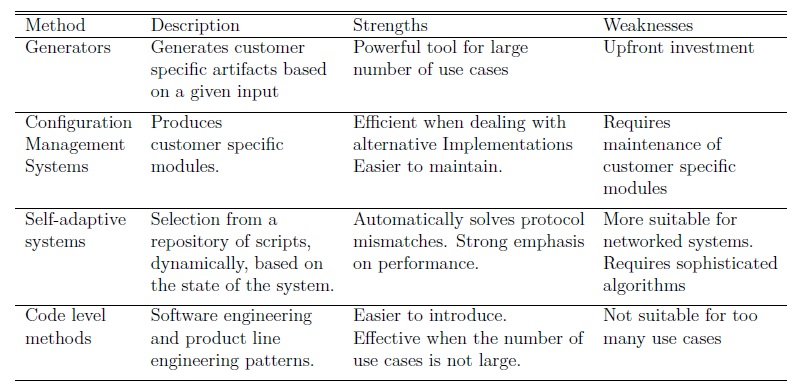
\includegraphics[width=.8\textwidth]{figure/figure14.jpg}
\caption{Summary of strengths and weaknesses of the main methods}
\label{fig:strenghtsWeaknesses}
\end{figure*}




A generator would require too significant upfront investment. Additionally, there are currently not enough identified use cases. Therefore, the return of investment can not be easily estimated. 

To make use of Configuration Management Tools include a cost of their purchase. Alternatively, the existing version control systems of the company could suffice. The problem of this approach is that maintaining a history of changes of each customer specific components and configuration still requires effort~\cite{Bachmann2001}.  %(Bachmann \& Bass 2001 p7). 
This technique could be a viable approach if there were more concrete use cases and there was an urgent need to maintain all these different components from the side of Jeppesen.

Self-adaptive systems is a more viable approach for networked systems. However, maintaining a knowledge-base where the appropriate script to handle a certain situation could be proved viable, especially for run time binding.

Code level techniques appear to be more suitable in the case of the investigated interface. The main argument to support this decision is that the number of possible customer specific requirements is not expected to be too high. There is a significant number of different techniques. %We choose to follow the general grouping discussed in (V�lter, 2009), which is the removal, injection and parametrization as we discussed in 3.7.4.2. 
For adopting a more concrete realization mechanism, we choose to follow the taxonomy of~\cite{JillesVanGurp2001}. % (Svahnberg, Gurp, Bosch 2005). 
In figure 5.4 we borrow their summary. The indicators which we discussed previously can help us choose among those methods. 



%\begin{figure*}[h]
%\centering
%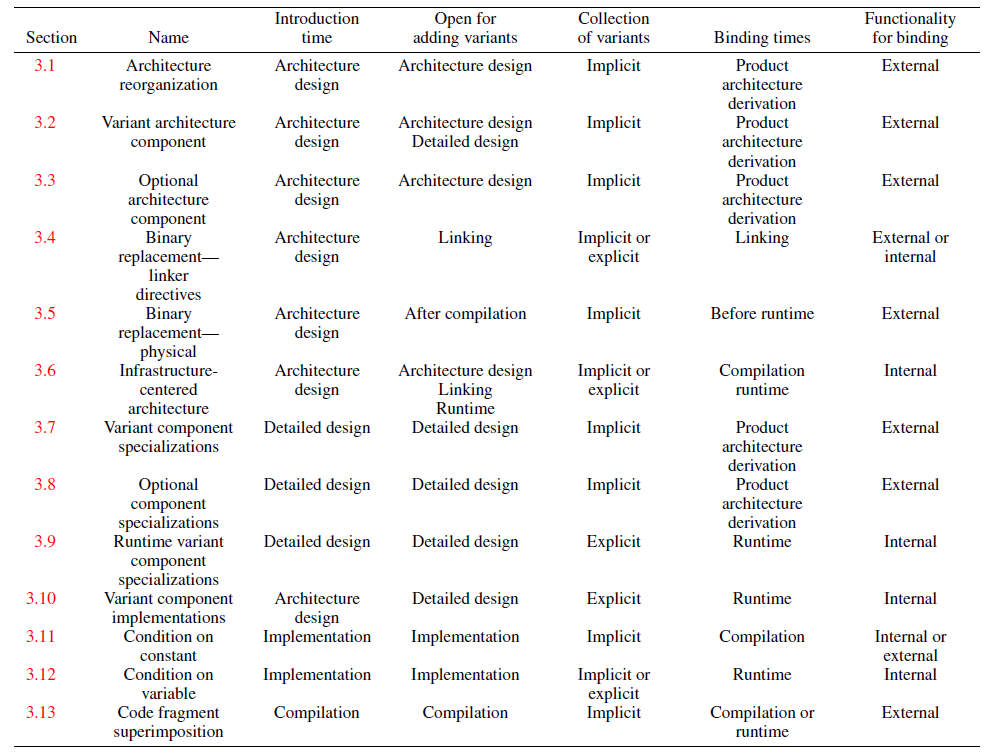
\includegraphics[width=1.0 \textwidth]{figure/figure3.png}
%
%\caption{ Summary of realization mechanisms. Taken from (Svahnberg, van Gurp \& Bosch, 2005 p742)}
%\end{figure*}

We preferred a solution which does not require major architectural restructuring, as this would interfere with the company's current approaches. For this reason, we focused on two techniques, \textit{Variant component} specializations and \textit{Optional component specializations} as they comply with the identified indicators. 
In the next chapter we provide more details about the method we choose to follow and the reasoning behind it. 

\section{Guidelines for decision making} 

We performed this study in a context in which the company does not follow traditional software product lines methods, as the customers are expected to edit and maintain code in the customization layer while the company is mostly responsible for the  maintenance of the core implementation. In every customization case, decisions need to be taken. In the following we report lessons learned stigmatized into guidelines in an attempt to support future customization decisions.
%The SSIM interface gave us a strong basis to perform our study. %Based on it, we document the guidelines in an attempt to support future customization decisions.

Each variation point needs to be dealt independently and in isolation. The characteristics of each point need to be identified; based on these, the decision of how it is going to be integrated in the system is taken. We therefore create a list of questions to ask so as to understand these characteristics, followed by a list of variability handling mechanisms. 

\subsection{Understanding the nature of the variation point} 

The first question is what is the likelihood that the variation point will appear more than once. Is it a special case required by only one customer or does it appear to multiple customers? 

The second questions is concerned with the collection of the variants and subsequently, the binding time. If the variation point is shared by all the customers, then the collection is explicit and it is bound in run time. 
However, if the collection is implicit, the system is modified accordingly in build time.

The third question is about the problem itself, whether it is a structural or a logical problem. A structural problem is concerned with translating the raw input in the correct semantics. A logical problem is concerned with how an algorithm manipulates the provided semantics.

Finally, one important question is about the estimated complexity of the code to deal with a variation point. This means, it could either be a rather simple to write script from scratch, or it could require a deeper understanding of the system's core code and strong programming skills.

%Is it rather simple to write a script from scratch, or does it understand a deeper understanding of the system's core code and good programming skills.
\subsection{Implementation of a variation point} 

Having defined the characteristics of the variation point, the next step is to decide how and where it should be implemented. Again, a few decisions need to be taken.

The first one is about who is expected to write code. If the expected complexity to implement a customer specific use case is expected to be low and it is unlikely that it will appear more than once, then it is up to the customers to write code. However, if the complexity is expected to be high, or the variation point is likely to appear more than once, then the company's engineers would need to develop a high-quality function.


Furthermore, if the problem type of the variation is a structural issue, the corresponding function could be encapsulated in the parser. If, on the other hand, it is a logical issue, an algorithm which provides diverse behaviour based on the given semantic input seems more of a reasonable option. 

Finally, a mechanism which allows the users to access the variation point should be defined. If the collection of variants is explicit and their binding is done in run time, then the variation point should be embodied in the core of the system. In the opposite case, where the collection of variants is implicit and the binding is done in build time, the variation point could be part of the customization layer. It could be implemented as a new function, part of a repository of scripts, where clients simply choose those needed for their needs. If the variation point can be simply replicated by calling a function but requires to modify the function itself, the variation point could take the form of documentation and coding standards. 



\section{ Conclusion}\label{sec:conclusion}

Software customization has an impact throughout all the software life cycle such as requirements elicitation, the design of the system, development, deployment and maintenance. The majority of the existing research is suggesting ways of how to support customizability where a company follows traditional product lines approaches and the variations will live very long. 

In the case of the company where this study was performed this was not the case. The company controls only the core part of the system and loses control of customer specific code. The customers are responsible for part of the code's maintenance. By the time the study took place, the company's newest system was hardly supporting two customers.

The aim of the study was to look further ahead and mitigate the risks which could potentially arise in the future. We explored the existing literature for methods, patterns and practices to suggest a way to handle variability in an easy, cheap and efficient way. 

We provided a trade-off analysis of the available methods. Furthermore, we documented the work flow and how we conceived the suggested method in our study. We ambition that the findings of this work will provide a strong basis to facilitate customization efforts by companies of similar technical contexts. 

The overall feedback we received  from the company's stakeholders suggested that our method will be integrated in the future by the company. We therefore encourage validation of the suggested methods through integration and the expansion of the guidelines of the decision making process. For this purpose, we have already pushed a repository containing a number of sample functions, ready to be used by the employees of the company.

 %Additionally, we suggested ways for future work in section 9.1. 
 %We do not expect that the findings of this study will either solve all the customization problems of the company, nor will they reshape the vast landscape of software customization.  We hope, however, that it will serve as a step forward to the vision of handling variability needs in an optimum way and add up to the existing knowledge for problems of similar nature. 
 



%\section{Future work} 





The evaluation of the proposed methods in this study were based on the feedback of various stakeholders of the company. To justify whether or not these methods would actually provide the expected benefits, integration with the company's new system is required. We hope that the prototype which we included in the company's code repository will be used by the employs and be validated further.



Additionally, the guidelines as well as the lessons learned of this study and similar projects should be retained in some way. A knowledge base could therefore facilitate the purpose of continuously improve and refine existent knowledge. Each project could be viewed as an opportunity to expand this knowledge repository. Furthermore, a knowledge base would provide robust guidelines to drive future customization decisions. Especially in combination of our method, this preserved knowledge could help the engineers to decide which method should be included in a script repository and which should be part of the customization layer for example. This knowledge base could also be expanded by asking people who worked with similar interfaces about their past experiences, worst cases they had and how they came up with certain solutions. 



Finally, another idea would be to develop some sort of interactive questionnaire. The purpose of this tool is to support the requirements elicitation for interfaces in a structured way, by suggesting the appropriate questions to ask their customers. It could guide the identification of important information such as the different use cases and their frequency of change. The initial content of this tool could be based on the findings of this study and by performing some interviews about the general desired requirements information and their priority. It could be extended with more questions based on the experience gained from interfacing projects.

We finally presented some ideas for future work. These triggered discussion among the stakeholders of how the company could support its customization needs more efficiently. One of these ideas was to maintain a knowledge repository. The stakeholders discussed about how sometimes do not know whether something should be in the customization layer or in the core, as there have been cases that were proven as more complex than originally thought or something appears second time and so on. Therefore, maintaining the knowledge of each project could support future decisions. However, they pointed that no one usually wants to work on it as it is viewed as a tedious task. The second idea for future work was an interactive questionnaire whose purpose would be to support the requirements elicitation by providing the right questions to ask their customers.




\section*{Acknowledgements}
\todo{software center and Jeppesen, in particulal Thekla}			

\balance

\bibliographystyle{IEEEtran}
\bibliography{bibliography}
%\nobalance

% CREATED BY DAVID FRISK, 2015
\section*{Appendix: Interview and evaluation questions}

\subsection*{Semi-structured interview questions} 

 \begin{enumerate}
  \item What is the translation process of the SSIM to semantics that your company understands?
  \item In your experience, can you give us examples where a field inside the SSIM was used in a different way from customer to customer? That is, customers had their own interpretation of that field? And why does this happen?
  
  
  
  
  \item What about with misinterpretations of the semantics, what could go wrong? And how often can it occur?
  \item What would you ask your customers to elicit their use cases?
  \item Tell us, according to your experiences, about parts of the IATA that could be misinterpreted, that could maybe be handled differently from different customers?
  
  \item How did you manage these issues in the past? 
  \item How are you handling things right now? Do you think there are issues with the current approach?

   
 \end{enumerate}



\subsection*{Group interview questions} 

For each of the following variation points we found during our analysis phase: \\

\begin{enumerate}
  \item  Do you agree that they are indeed a variation point?
  \item  Is there something else that we might have missed?
  \item What do you think is the most urgent to deal with? 
  
  
  \end{enumerate}

\subsection*{Code analysis questions} 

\begin{enumerate}
\item Can you guide us through the SSIM integrator's code of the old system?
\item Can you talk a little about the special cases the integrator is handling?
\item Can you elaborate more about special cases of your customers?
\item Do you have other issues with the interpretations of the semantics?
\item How do you detect these misinterpretations? and how do you handle them?

  \end{enumerate}

\subsection*{First evaluation questions}



\begin{enumerate}
\item The functions that you wrote for your current customer in the new system, do you think they can be reused by some other airline?

\item Do you think, in general, that certain use cases might appear to other customers?

\item (after presenting our suggested method) Do you think this approach is good or bad? Why? 

\item Are there some other ways that you could suggest for handling customer specific use cases?

\item Do you think this method could be replicated to other contexts as well?

\item Would you consider integrate this?

  \end{enumerate}

\subsection*{Final evaluation questions} 
\begin{enumerate}
\item What do you think of this approach? And Why? Do you agree with the preliminary feedback? 

\item Do you think use recurring customer specific use cases could emerge for the SSIM interface? What about other interfaces? 

\item What guarantee you have that your customers will write quality code and that their systems will be compatible with yours? 

\item How do your customers understand the system's core and how do they test it?

\item Do you agree with these guidelines? And Why? Is there something missing? 

\item (after discussing variability management for the Operational Messages interface) Do you agree with this approach? And Why? 

\item What do you think about possible future work? What other ways could support the understanding and effective management of variability? 


  \end{enumerate}




\end{document}